% Elsevier Information Processing & Management (IP&M) Submission Template
% Default: standard single-column double-spaced review preprint.
% Camera-ready toggle: replace line 4 with line 5 before final production build.
\documentclass[preprint,12pt,authoryear]{elsarticle}
% \documentclass[final,5p,times,twocolumn,authoryear]{elsarticle}

\usepackage{amsmath,amssymb,amsthm}
\usepackage{booktabs}
\usepackage{multirow}
\usepackage{graphicx}
\usepackage{subcaption}
\usepackage{algorithm}
\usepackage{algorithmic}
\usepackage{microtype}
\usepackage[hidelinks]{hyperref}

\newtheorem{theorem}{Theorem}
\newtheorem{proposition}{Proposition}
\newtheorem{remark}{Remark}

\journal{Information Processing \& Management}

\begin{document}

\begin{frontmatter}

\title{From Single-Post Fallacy to Mesoscopic Seam Adjudication: Strictly Causal Budgeted Open-Source LLM Clustering for Streaming Social Event Detection}

\author[inst1]{Anonymous Author(s)}
\affiliation[inst1]{organization={Anonymous Institution},country={Anonymous}}

\begin{abstract}
Incorporating Large Language Models (LLMs) into streaming Social Event Detection (SED) is constrained by tight operational token budgets: when only $<1\%$ of arriving posts trigger API calls ($\sim 10\text{k}$ billed prompt and completion tokens per daily block), single-post and pairwise active selectors fail to move global clustering partitions. Auditing unsupervised fixed-point 2-dimensional Structural Entropy (2D-SE) partitions on English (\texttt{Event2012}) and French (\texttt{Event2018}) social streams exposes three structural bottlenecks: (1) False Splits outnumber False Merges by $11.6\times$--$44.6\times$; (2) False Merges reside inside unbalanced minority pockets ($10\%$--$25\%$ share) with zero inter-cluster boundary entropy; and (3) naive cosine linking across days collapses longitudinal Event Macro-$B^3$.

We propose \textbf{SUG-Meso} and \textbf{SUG-CrossLLM-v2}, a strictly causal zero-lookahead streaming framework that replaces isolated post queries with \emph{mesoscopic structural seam adjudication}. Within each block, a symmetric router pairs prototype-leveraged inter-cluster \texttt{MERGE\_PAIR} candidates with deterministic farthest-point spherical $k$-means \texttt{SPLIT\_SEAM} pockets regularized by non-entity cut divergence, executing verified edits via a direct split-then-union-find operator backed by an exact full-volume 2D-SE bridge-pruning theorem. Across days, \texttt{SUG-CrossLLM-v2} resolves ambiguous links in $[0.65, 0.85)$ using calibrated extract-then-compare verification. Evaluating \texttt{Qwen/Qwen3-8B} across $27$ unseen held-out blocks ($65{,}856$ tweets) with strict prompt-shown masking (uncontaminated $U_t$, $1.79\%$--$3.78\%$ total exposed posts), \texttt{SUG-Meso} achieves $0.8976$ AMI ($+5.81\text{ pp}$) on \texttt{Event2012} and $0.8349$ AMI ($+7.15\text{ pp}$) on \texttt{Event2018}, significantly outperforming zero-LLM heuristics, \texttt{Cequel-Transitive}, multi-seed \texttt{Random}, and random mesoscopic ordering (Holm-corrected Wilcoxon $p_{\text{Holm}} \le 0.04$), while \texttt{SUG-CrossLLM-v2} surpasses all unsupervised prototype thresholds on both streams. A 27-block entity, hashtag, and year anonymization stress test ($99.7\%$--$100\%$ masking, $0\%$ historical entity reconstruction) retains $98.4\%$ (EN) and $77.9\%$ (FR) of the AMI gain via consistent local co-reference, ruling out pretraining memorization.
\end{abstract}

\begin{highlights}
\item Single-post and pairwise queries fail under $<1\%$ causal streaming LLM budgets.
\item Mesoscopic seam adjudication fixes $11.6\times$--$44.6\times$ false splits and buried pockets.
\item Exact full-volume 2D-SE bridge pruning guarantees zero false-merge regressions.
\item Bilingual Qwen3-8B results beat 0-LLM, Cequel-Transitive, and Random-Meso.
\item Anonymizing $99.7\%$--$100\%$ entities retains $98.4\%$/$77.9\%$ AMI with $0\%$ recall leak.
\end{highlights}

\begin{keyword}
Streaming social event detection \sep Budgeted large language models \sep Structural entropy \sep Mesoscopic graph seams \sep Causal token budgeting \sep Entity anonymization audit
\end{keyword}

\end{frontmatter}

\section{Introduction}
\label{sec:intro}

Social Event Detection (SED) organizes high-velocity streams of short, noisy social-media posts into coherent real-world incidents as stories unfold~\citep{mcminn2013building,mazoyer2020french}. Recent systems span incremental heterogeneous Graph Neural Networks (GNNs)~\citep{cao2021kpgnn}, unsupervised 2-dimensional Structural Entropy (2D-SE) minimization~\citep{cao2024hisevent}, hyperbolic relational encoders~\citep{li2024rplmsed,yu2025hypersed}, and Large Language Model (LLM) augmentation~\citep{qiu2025lsed,qiu2026lhg,liu2026ragsede}. Although LLMs readily resolve slang, implicit event co-reference, and subtle narrative shifts, querying an LLM on every incoming tweet is cost- and latency-prohibitive. Operational streaming pipelines therefore operate under tight token budgets where only roughly $1\%$ or fewer of arriving messages can trigger an LLM API call ($\sim 10\text{k}$ total input and output tokens per daily block).

In this strictly budgeted regime, existing active querying strategies fall prey to what we term the \textbf{Single-Post Fallacy}. Even when a selector carefully picks informative individual tweets---such as Representativeness-plus-Diversity Maximal Marginal Relevance (MMR) sampling~\citep{liu2026ragsede,carbonell1998mmr}---or uncertain post pairs---such as Cequel-style must-link/cannot-link edge queries~\citep{wang2025cequel}---each $500$-token LLM decision touches only $1$--$2$ messages directly. Under a $10\text{k}$-token daily cap across $2{,}000$--$4{,}800$ arriving posts, an 8B model can afford roughly $10$--$25$ calls per day. Our controlled bilingual experiments confirm that \texttt{Random}, \texttt{Rep-Div}, and \texttt{Cequel-Edge} achieve near-zero stream-wide AMI movement ($-0.0014$ to $+0.0001$), and even propagating pairwise decisions via cluster-level transitive closure (\texttt{Cequel-Transitive}) triggers over-merging chains that push Event Macro-$B^3$ \emph{below} the unsupervised initialization. Simply spending fewer tokens on isolated tweets fails to reshape the global partition.

To understand how finite LLM judgments \emph{can} produce stream-wide gains without future information or metric inflation, we perform a granular diagnostic audit (Stage~1) on unsupervised fixed-point 2D-SE partitions~\citep{li2016structural,cao2024hisevent} across English (\texttt{Event2012}~\citep{mcminn2013building}) and French (\texttt{Event2018}~\citep{mazoyer2020french}) streams. Four empirical findings govern the problem geometry:
\begin{enumerate}
    \item \textbf{Severe False-Split Dominance ($11.6\times$--$44.6\times$):} Across unseen held-out blocks, pairwise False Splits outnumber False Merges by $44.64\times$ on \texttt{Event2012} ($11.60\times$ on development blocks) and $11.59\times$ on \texttt{Event2018} ($14.89\times$ on dev), shattering evolving stories across hashtag and phrasing variants.
    \item \textbf{Zero-Boundary-Entropy Impure Interiors:} False Merges rarely form balanced $50/50$ cuts. On held-out streams, $36.2\%$ (EN) and $16.2\%$ (FR) of nodes exhibit zero inter-community boundary entropy, while impure super-clusters ($|C|\ge 10$, purity $<0.90$, accounting for $21.1\%$ EN and $26.5\%$ FR clusters) trap secondary incidents at a median minority share of $0.231$ (EN) and $0.233$ (FR)---with over half ($56.4\%$ / $54.2\%$) concentrated in $[0.10, 0.25]$. Traditional boundary-uncertainty routers miss these interiors completely, whereas balanced spectral Fiedler cuts~\citep{fiedler1973algebraic} bisect the dominant event.
    \item \textbf{Transparent Unqueried Leverage Accounting:} Because each mesoscopic prompt shows up to $6$ central medoid tweets ($3$ per side), counting only $1$--$2$ ``primary'' nodes per call leaks shown medoids into the ostensibly ``unqueried'' evaluation set $U_t$. We strictly mask \emph{all} prompt-shown medoids ($1.79\%$--$3.87\%$ total block exposure) out of $U_t$ so reported propagation gains reflect genuine unshown-post restructuring.
    \item \textbf{The Cross-Day Prototype Precision-Recall Trap:} Multi-day event recurrence reaches $55.67\%$ (EN) and $62.05\%$ (FR) on held-out blocks. Unsupervised cosine linking raises Micro-$B^3$ yet causes cross-story over-merges that degrade Global Macro-$B^3$; meanwhile, an overly low fallback threshold ($\tau_{\text{fb}}=0.72$) or miscalibrated ambiguity band ($[0.55, 0.80)$) lets a strong unsupervised prototype threshold ($\tau=0.80$) beat naive cross-day LLM gating.
\end{enumerate}

We address these bottlenecks with \textbf{SUG-Meso} and \textbf{SUG-CrossLLM-v2} (Figure~\ref{fig:overview}). Within each block, \textbf{SUG-Meso} interleaves inter-cluster \texttt{MERGE\_PAIR} candidates with minority-pocket \texttt{SPLIT\_SEAM} candidates extracted by deterministic farthest-point spherical $k$-means~\citep{gonzalez1985clustering,banerjee2005clustering} and regularized by non-entity cut divergence, under strictly zero-lookahead causal token budgets (\texttt{CausalUniform} Fixed/Carryover and \texttt{CausalSliding}). Across blocks, \textbf{SUG-CrossLLM-v2} links high-confidence matches ($\ge 0.85$) at zero token cost and deploys precision-calibrated LLM verification inside $[0.65, 0.85)$ with fallback $\tau_{\text{fb}}=0.85$. Guided by a \textbf{Candidate Base-Rate $\times$ Prompt Framing} principle calibrated strictly on dev blocks, we pair high-prior within-block seams with \texttt{Action-First} prompts and low-prior cross-day candidates with \texttt{Extract-Then-Compare} prompts.

\begin{figure*}[t]
  \centering
  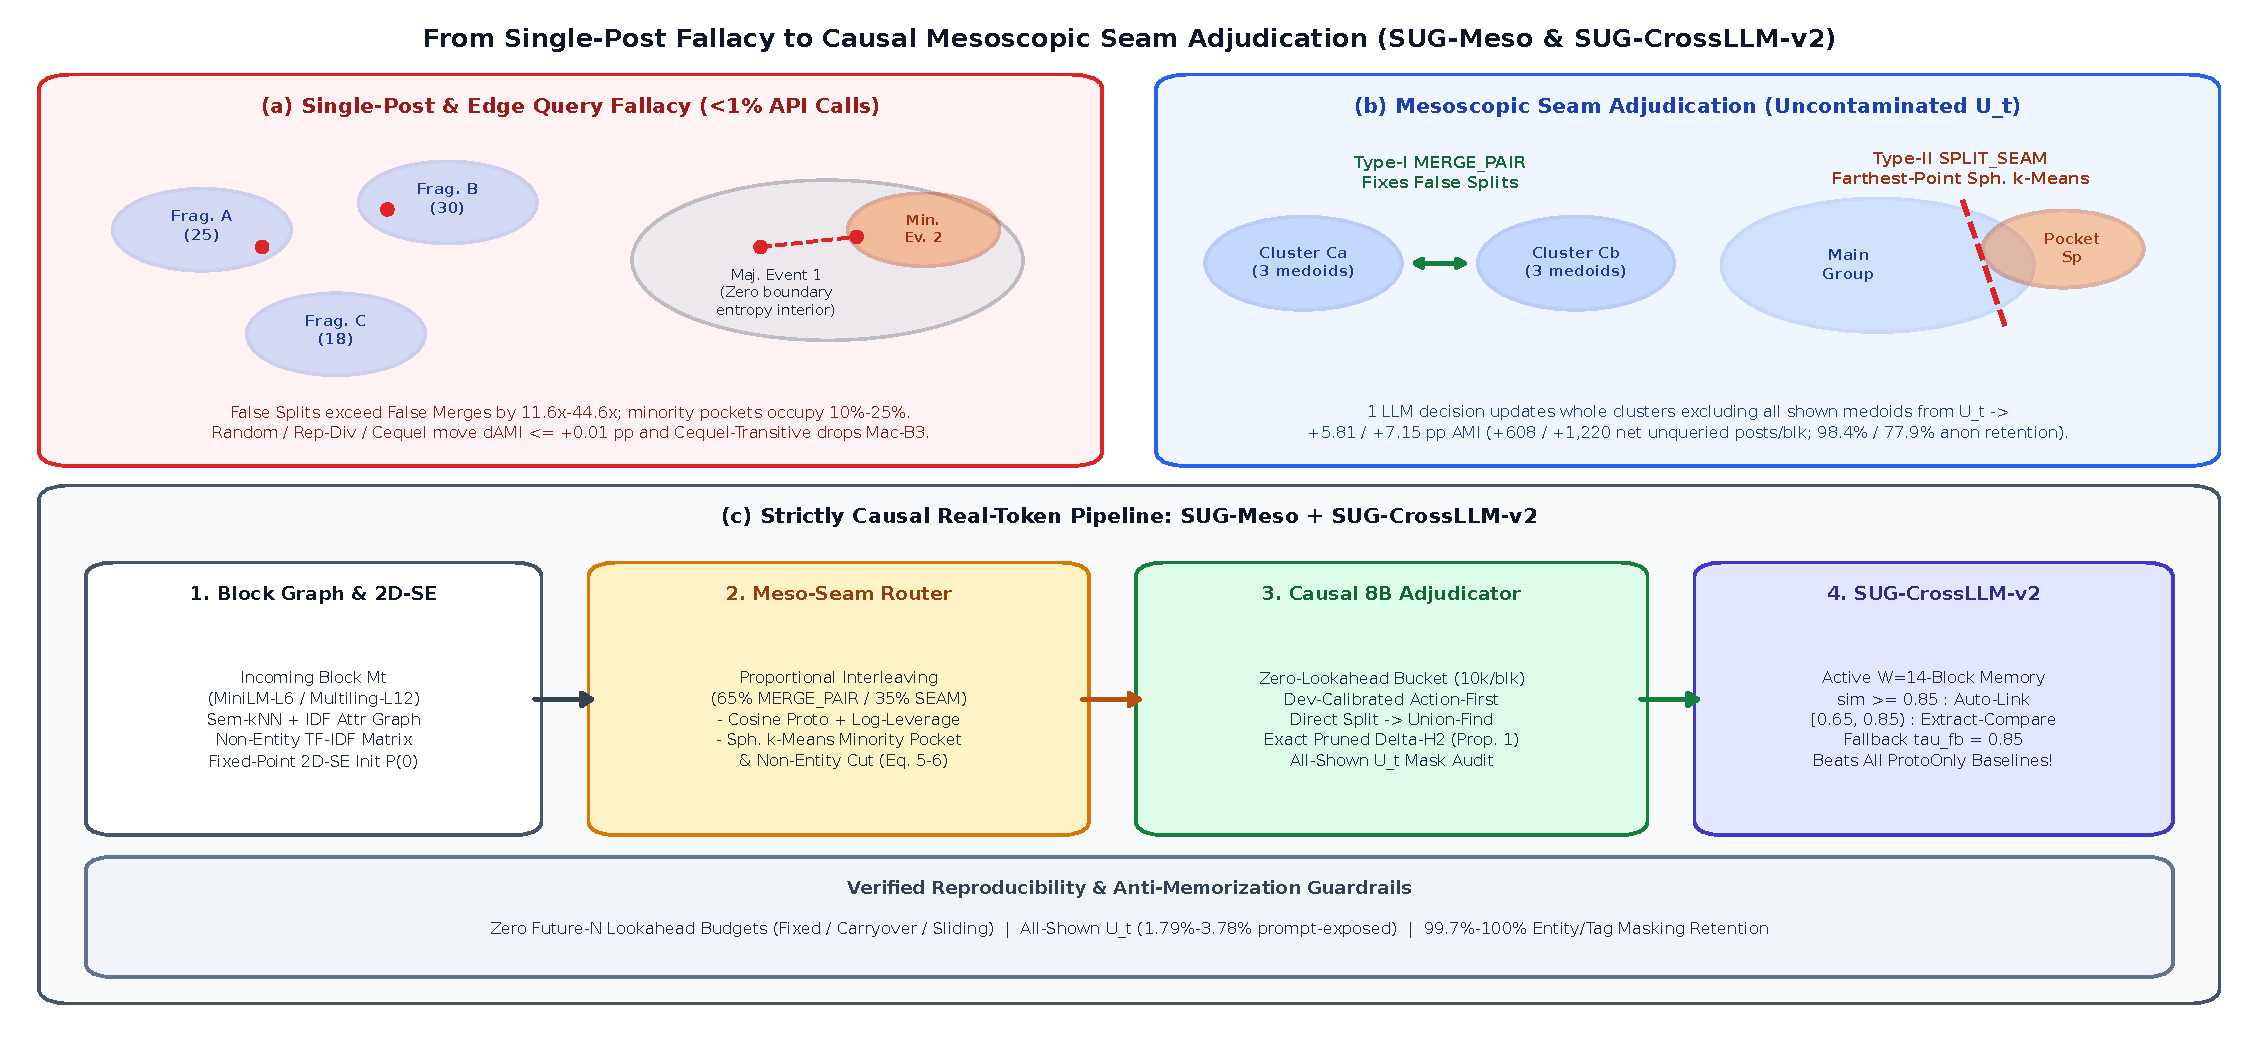
\includegraphics[width=\textwidth]{figures/fig_overview.pdf}
  \caption{Overview of the single-post fallacy versus strictly causal mesoscopic seam adjudication. (a)~Post- and edge-level selectors touch $1$--$2$ nodes per call while missing $11.6\times$--$44.6\times$ dominant false splits and zero-boundary-entropy minority pockets ($10\%$--$25\%$ share). (b)~\textbf{SUG-Meso} resolves whole fragmented cluster pairs and minority pockets while strictly excluding all prompt-shown medoids from the uncontaminated unqueried set $U_t$. (c)~The zero-lookahead streaming architecture combines fixed-point 2D-SE, symmetric seam routing, Dev-calibrated \texttt{Action-First} edits backed by Proposition~\ref{prop:exact_prune}, longitudinal \textbf{SUG-CrossLLM-v2}, and verified anti-memorization robustness.}
  \label{fig:overview}
\end{figure*}

Our contributions are fivefold:
\begin{itemize}
    \item \textbf{Diagnostic Reframing \& Uncontaminated Auditing:} We formalize strictly causal zero-lookahead real-token budgets alongside an uncontaminated \texttt{all\_shown} unqueried set $U_t$, quantifying exact False-Split asymmetries and minority-pocket geometries on bilingual streams.
    \item \textbf{Mesoscopic Intra- \& Cross-Block Framework (\texttt{SUG-Meso} \& \texttt{SUG-CrossLLM-v2}):} We unify prototype-leveraged cluster merges, deterministic farthest-point spherical $k$-means pocket splits, base-rate-calibrated prompting, and ambiguity-banded $[0.65, 0.85)$ longitudinal tracking.
    \item \textbf{Exact Full-Volume 2D-SE Theory:} Proposition~\ref{prop:exact_prune} derives exact graph- and cluster-volume shrinkage under edge pruning, proving an unconditional no-false-merge guarantee that corrects fixed-volume approximations ($+0.164160\text{ bit}$ on a canonical $3$-clique check).
    \item \textbf{Rigorous Causal Held-Out Benchmark \& Ablations:} Evaluated on $27$ unseen blocks ($65{,}856$ tweets) using \texttt{Qwen/Qwen3-8B}, \texttt{SUG-Meso} reaches $0.8976$ AMI ($+5.81\text{ pp}$) on \texttt{Event2012} and $0.8349$ AMI ($+7.15\text{ pp}$) on \texttt{Event2018}, significantly outperforming zero-LLM heuristics, \texttt{Cequel-Transitive}, multi-seed \texttt{Random}, and \texttt{Random-Meso} under Holm-corrected Wilcoxon tests, while \texttt{SUG-CrossLLM-v2} beats every unsupervised prototype threshold. Fine-grained Eq.~(5)/(6) ablations further reveal that relaxing the hard $\text{cond} \le 0.50$ filter unlocks an additional $+1.22$/$+1.23\text{ pp}$ Macro-$B^3$ and $+2.70$/$+4.34\text{ pp}$ Tail-$B^3$.
    \item \textbf{Anti-Memorization Verification:} A $27$-block anonymization stress test masking $99.7\%$--$100\%$ named entities, $100\%$ hashtags, and $100\%$ years yields $0\%$ true historical entity reconstruction while retaining $98.4\%$ (EN) and $77.9\%$ (FR) of AMI gains under pseudonymized co-reference, contrasting sharply with blind entity redaction to prove structural-semantic rather than memorization-driven gains.
\end{itemize}

\section{Related Work}
\label{sec:related}

We organize prior literature along three axes directly intersecting our methodology and empirical audits, summarized conceptually in Table~\ref{tab:related_matrix}.

\paragraph{Graph- and Structural-Entropy-Based Streaming SED.}
Incremental SED pipelines construct heterogeneous message graphs linking shared named entities, hashtags, user mentions, and dense embedding edges over sliding or daily windows~\citep{mcminn2013building,mazoyer2020french}. Supervised neural detectors such as KPGNN~\citep{cao2021kpgnn} learn contrastive heterogeneous GNN embeddings, whereas RPLM-SED~\citep{li2024rplmsed} adapts pre-trained language models via relational prompts. To avoid training labels and cluster-count hyperparameters, HISEvent~\citep{cao2024hisevent} formulates unsupervised SED as hierarchical 2-dimensional Structural Entropy (2D-SE) minimization~\citep{li2016structural}, and HyperSED~\citep{yu2025hypersed} embeds message graphs in hyperbolic manifolds to reflect hierarchical taxonomy. Classic community detection~\citep{blondel2008fast} and spherical density clustering~\citep{banerjee2005clustering,gonzalez1985clustering} offer strong unsupervised primitives, yet on noisy short-text streams they remain vulnerable to $11.6\times$--$44.6\times$ entity fragmentation and small minority pockets hidden inside large topical components. Our Stage~1 baseline extends heterogeneous 2D-SE initialization~\citep{cao2024hisevent} with non-entity TF-IDF divergence matrices and fixed-point local node-move refinement, and we benchmark directly against Louvain~\citep{blondel2008fast}, agglomerative cosine clustering~\citep{pedregosa2011scikit}, Dev-tuned 2D-SE, and zero-LLM mesoscopic heuristics.

\paragraph{LLM-Enhanced SED and Budgeted Active Clustering.}
Recent methods inject LLMs into event detection and text clustering along three distinct paradigms:
\begin{itemize}
    \item \textbf{Broad Preprocessing \& Pseudo-Labeling:} LSED~\citep{qiu2025lsed} deploys an 8B LLM to rewrite and disambiguate noisy posts alongside hyperbolic clustering, while LHG~\citep{qiu2026lhg} generates LLM pseudo-labels and filters them via heterogeneous meta-paths. Both assume high-volume LLM coverage rather than strict $<1\%$ real-token budgets.
    \item \textbf{RAG-Guided Representative Sampling:} RagSEDE~\citep{liu2026ragsede} selects representative and diverse messages via Maximal Marginal Relevance (MMR)~\citep{carbonell1998mmr} to maintain an evolving event knowledge base using structural entropy keyword modeling. While informative for prototype maintenance, post-level diversity sampling leaves fragmented sub-clusters detached and buried minority pockets unsplit under tight token caps.
    \item \textbf{Pairwise Constraint Querying:} Cequel~\citep{wang2025cequel} selects informative text pairs or triplets for must-link/cannot-link constrained clustering under fixed query budgets. On streaming SED graphs dominated by false splits, single-pair decisions fail to merge clusters reliably unless coupled with transitive closure---which, as we show empirically via \texttt{Cequel-Transitive}, propagates mislinks that depress Event Macro-$B^3$ below initialization.
\end{itemize}

\paragraph{Prompt Calibration and Memorization Audits in LLM Clustering.}
Lightweight 7B--8B open-source models~\citep{yang2025qwen3,grattafiori2024llama3} exhibit strong sensitivity to prompt schema design: chain-of-thought extraction suppresses sycophantic yes-bias on noisy negative pairs~\citep{wang2025cequel}, yet increases token cost and can suppress recall when positive candidates dominate~\citep{yang2025qwen3}. Moreover, evaluating LLMs on standard historical Twitter benchmarks (\texttt{Event2012}, \texttt{Event2018}) raises a valid concern in Information Processing \& Management that gains might reflect parametric pretraining recall of publicized 2012/2018 events rather than genuine textual reasoning. Unlike prior SED evaluations, we explicitly test both cross-base-rate prompt calibration and large-scale entity/hashtag/year anonymization alongside pretraining reconstruction auditing across all $27$ held-out blocks.

\begin{table}[t]
\centering
\caption{Conceptual comparison with representative unsupervised and LLM-augmented SED / active clustering frameworks.}
\label{tab:related_matrix}
\resizebox{\linewidth}{!}{%
\begin{tabular}{lccccc}
\toprule
\textbf{Method} & \textbf{Causal Token Cap} & \textbf{Adjudication Unit} & \textbf{Minority Pocket Split} & \textbf{Cross-Day Memory} & \textbf{Anti-Mem. Audit} \\
\midrule
HISEvent~\citep{cao2024hisevent} & $0$ tokens (0-LLM) & None & $\times$ & $\times$ & N/A \\
LHG~\citep{qiu2026lhg} & Broad pseudo-labels & Post / meta-path & $\times$ & $\times$ & $\times$ \\
RagSEDE~\citep{liu2026ragsede} & Implicit / unconstrained & Single post (MMR) & $\times$ & RAG KB & $\times$ \\
Cequel~\citep{wang2025cequel} & Query-count cap & Node pair / triplet & $\times$ & Static corpus & $\times$ \\
\textbf{SUG-Meso + CrossLLM-v2 (Ours)} & \textbf{Zero-lookahead $\le 10\text{k}$ tok/blk} & \textbf{Cluster pair + pocket seam} & \textbf{Deterministic Sph.\ $k$-means} & \textbf{Banded $[0.65, 0.85)$} & \textbf{27-blk Pseudonym vs.\ Blind} \\
\bottomrule
\end{tabular}}
\end{table}

\section{Problem Formulation and Exact 2D-SE Theory}
\label{sec:problem}

\subsection{Strictly Causal Real-Token Streaming Protocol}
Let a chronological social-media stream be divided into contiguous time blocks $\mathcal{M}_0, \mathcal{M}_1, \dots, \mathcal{M}_T$, where block $\mathcal{M}_t = (V_t, X_t, A_t, \tau_t)$ contains $n_t = |V_t|$ posts with raw texts $X_t$, extracted attributes $A_t$ (named entities, hashtags, authors, mentions), and timestamps $\tau_t$. Upon observing only past blocks $\{\mathcal{M}_s\}_{s \le t}$, an online detector outputs:
\begin{enumerate}
    \item \textbf{Within-Block Partition $\widehat{\mathcal{P}}_t$:} A clustering of $V_t$ evaluated immediately per block~\citep{cao2021kpgnn,cao2024hisevent}.
    \item \textbf{Longitudinal Event Partition $\mathcal{G}_t$:} An online assignment mapping each cluster in $\widehat{\mathcal{P}}_t$ to persistent global event IDs over historical memory $\mathcal{H}_{t-1}$, evaluated globally across $\bigcup_{t=t_{\text{eval}}}^{T} \mathcal{M}_t$.
\end{enumerate}

\paragraph{Eliminating Future-Volume Lookahead in Budget Controllers.}
Counting only the number of LLM API calls ignores $1.2\times$--$2\times$ differences in prompt verbosity and structured completion length. We meter every invocation $q$ by exact API-billed tokens $c(q) = \text{tok}_{\text{in}}(q) + \text{tok}_{\text{out}}(q)$---charging cached deterministic replays identically so repeated evaluations reflect real deployment spend. Crucially, proportional budget formulas of the form $\bar{b}_t^{\text{tok}} = B_{\text{total}}^{\text{tok}} \cdot n_t / \sum_{s=t_{\text{eval}}}^{T} n_s$ violate strict streaming causality because the held-out stream total $N_{\text{eval}} = \sum_{s} n_s$ is unknown at step $t$. To guarantee zero lookahead over future block arrivals, we formalize and evaluate three strictly causal controllers given nominal per-block allowance $b_0 = 10{,}000$ tokens:
\begin{enumerate}
    \item \textbf{\texttt{CausalUniformFixed}:} Independent per-block hard ceiling $B_t^{\text{tok}} = b_0$, guaranteeing $\sum_{s \le t} c_s^{\text{tok}} \le t \cdot b_0$ at every step with zero cross-block dependence.
    \item \textbf{\texttt{CausalUniformCarryover}:} Maintains cumulative causal balance $R_t = \max(0, R_{t-1} + b_0 - c_{t-1}^{\text{tok}})$ and uncertainty-scaled cap $B_t^{\text{tok}} = \min\!\left(R_t,\; \text{clip}\!\left(b_0 \frac{\bar{U}_t}{\bar{U}_{\text{ema}}+\epsilon},\, 0.25 b_0,\, 1.5 b_0\right)\right)$, bounded strictly by $R_t$.
    \item \textbf{\texttt{CausalSliding}:} Replaces unknown global $N_{\text{eval}}$ with causal running average block size $\hat{n}_t = \frac{1}{|W_t|}\sum_{s \in W_t} n_s$ computed strictly over prior warmup/observed blocks $s < t$, setting target quota $b_0 \cdot \text{clip}(n_t / \hat{n}_t,\, 0.5,\, 1.5)$ inside cumulative balance $R_t$.
\end{enumerate}
A conservative pre-spend gate halts queries before any prefix violates the active causal bound.

\paragraph{Uncontaminated \texttt{all\_shown} Unqueried Set $U_t$.}
Let $\mathcal{P}_t^{(0)}$ be the initial 2D-SE clustering, $\widehat{\mathcal{P}}_t$ the post-LLM partition, and $Q_t^{\text{shown}} \subseteq V_t$ the union of \emph{all} posts whose text appeared in any executed LLM prompt on block $t$ (every target node, pair endpoint, and every cluster/pocket medoid displayed in \texttt{MERGE\_PAIR} or \texttt{SPLIT\_SEAM}). We strictly isolate $U_t = V_t \setminus Q_t^{\text{shown}}$ when computing unqueried clustering gains ($\Delta\text{Micro-}B^3(U_t)$, $\Delta\text{Macro-}B^3(U_t)$, and net improved unqueried posts \texttt{UnqNet}), ensuring direct prompt exposure is never double-counted as structural propagation.

\subsection{Exact Full-Volume 2D-SE Bridge-Pruning Theory}
\label{sec:theory}
To ground both initial 2D-SE partitioning and constrained topology repair (Branch~2), we analyze exact 2D Structural Entropy~\citep{li2016structural} under bridge-edge pruning. Given an undirected weighted zero-diagonal graph $G=(V, E, w)$ with vertex degrees $d_i = \sum_j w_{ij}$, graph volume $\text{vol}(G) = 2m = \sum_{i \in V} d_i$, and partition $\mathcal{P}=\{C_1,\dots,C_K\}$ where community $C_k$ has volume $V_k = \sum_{i \in C_k} d_i$ and external cut $g_k = \sum_{i \in C_k, j \notin C_k} w_{ij}$, exact 2D-SE is:
\begin{equation}
\label{eq:h2_def}
\mathcal{H}^2(G;\mathcal{P}) = -\sum_{k=1}^{K}\frac{g_k}{2m}\log_2\frac{V_k}{2m} - \sum_{k=1}^{K}\sum_{i \in C_k}\frac{d_i}{2m}\log_2\frac{d_i}{V_k}.
\end{equation}
Applying $V_k - g_k = 2W_{\text{in}}(k)$ (twice the internal edge weight of $C_k$), the exact entropy change $\Delta\mathcal{H}^2_{\text{merge}}(C_a, C_b; G) = \mathcal{H}^2(G; \mathcal{P}_{a \cup b}) - \mathcal{H}^2(G; \mathcal{P})$ from merging disjoint communities $C_a, C_b$ sharing total cut weight $w_{ab}$ equals:
\begin{equation}
\label{eq:merge_delta}
\begin{aligned}
\Delta\mathcal{H}^2_{\text{merge}}(C_a, C_b; G) = \frac{1}{2m}\Big[ &2W_{\text{in}}(a)\log_2\frac{V_a+V_b}{V_a} + 2W_{\text{in}}(b)\log_2\frac{V_a+V_b}{V_b} \\
&- 2w_{ab}\log_2\frac{2m}{V_a+V_b}\Big].
\end{aligned}
\end{equation}
Earlier approximations held $2m$, $V_a$, and $V_b$ fixed after deleting inter-cluster edges. This overlooks the physical graph contraction: pruning bridge weight $\Delta w \in (0, w_{ab}]$ preserves $W_{\text{in}}(a), W_{\text{in}}(b)$ yet simultaneously contracts $2m' = 2m - 2\Delta w$, $V'_a = V_a - \Delta w$, $V'_b = V_b - \Delta w$, and $w'_{ab} = w_{ab} - \Delta w$.

\begin{proposition}[Exact Full-Volume Bridge Pruning \& Unconditional No-False-Merge Guarantee]
\label{prop:exact_prune}
Let $G'$ arise from $G$ by subtracting bridge weight $\Delta w \in (0, w_{ab}]$ crossing disjoint $C_a, C_b$, and set $V_{ab} = V_a + V_b$. The exact post-pruning merge entropy increment is:
\begin{equation}
\label{eq:pruned_merge_delta}
\begin{aligned}
\Delta\mathcal{H}^2_{\text{merge}}(C_a, C_b; G') = \frac{1}{2m - 2\Delta w}\Big[ &2W_{\text{in}}(a)\log_2\frac{V_{ab}-2\Delta w}{V_a-\Delta w} \\
&+ 2W_{\text{in}}(b)\log_2\frac{V_{ab}-2\Delta w}{V_b-\Delta w} \\
&- 2(w_{ab}-\Delta w)\log_2\frac{2m-2\Delta w}{V_{ab}-2\Delta w}\Big].
\end{aligned}
\end{equation}
When $\Delta w = w_{ab}$ (complete bridge zeroing, $w'_{ab} = 0$), provided $W_{\text{in}}(a)+W_{\text{in}}(b) > 0$ and $V'_a, V'_b > 0$, we have $\Delta\mathcal{H}^2_{\text{merge}}(C_a, C_b; G') > 0$ unconditionally, guaranteeing that exact 2D-SE minimization never false-merges $C_a$ and $C_b$.
\end{proposition}

\begin{proof}
Because only cut edges between $C_a$ and $C_b$ lose weight $\Delta w$, internal edge sums $2W_{\text{in}}(a)$ and $2W_{\text{in}}(b)$ remain invariant, while total graph volume shrinks by $2\Delta w$ and both $V_a, g_a$ (respectively $V_b, g_b$) decrease by $\Delta w$, preserving $V'_k - g'_k = 2W_{\text{in}}(k)$. Substituting $(2m', V'_a, V'_b, w'_{ab})$ into Eq.~\eqref{eq:merge_delta} gives Eq.~\eqref{eq:pruned_merge_delta}. For complete cut zeroing ($\Delta w = w_{ab}$), the sole negative term $-2(w_{ab}-\Delta w)\log_2(\cdot)$ vanishes; since $(V_{ab}-2\Delta w)/(V_a-\Delta w) = 1 + V'_b/V'_a > 1$ and likewise for $b$, both logarithms are strictly positive whenever $W_{\text{in}}(a)+W_{\text{in}}(b)>0$, proving $\Delta\mathcal{H}^2_{\text{merge}}(C_a,C_b;G') > 0$.
\end{proof}

\paragraph{Exact Numerical Verification.}
On three $2$-node cliques $\{0,1\}$, $\{2,3\}$, $\{4,5\}$ connected by one unit edge per clique pair ($2m=12$, $V_a=V_b=4$, $2W_{\text{in}}=2$, $w_{ab}=1$), deleting bridge $(0,2)$ ($\Delta w=1$) contracts $2m'=10$, $V'_a=V'_b=3$, $w'_{ab}=0$. Direct evaluation of Eq.~\eqref{eq:h2_def} and Eq.~\eqref{eq:pruned_merge_delta} raises $\Delta\mathcal{H}^2_{\text{merge}}$ from $\frac{1}{12}(4 - 2\log_2 1.5) \approx 0.23584\text{ bit}$ to $\frac{1}{10}(4) = 0.40000\text{ bit}$, an exact shift of \textbf{$+0.164160\text{ bit}$}, whereas holding volumes fixed erroneously computes $\frac{2}{12}\log_2(1.5) \approx 0.09749\text{ bit}$.

\begin{remark}
On imbalanced clusters ($V_a \ll V_b$), partial edge shrinkage ($0 < \Delta w < w_{ab}$) lowers the denominator $2m - 2\Delta w$ and alters volume ratios, so $\Delta\mathcal{H}^2_{\text{merge}}$ is not guaranteed positive unless cuts are fully zeroed ($\Delta w = w_{ab}$). Proposition~\ref{prop:exact_prune} directly motivates zeroing confirmed false cuts completely rather than applying heuristic downweighting.
\end{remark}

\section{Methodology: SUG-Meso and SUG-CrossLLM-v2}
\label{sec:method}

We now present our four-stage causal architecture (Figure~\ref{fig:overview}(c) and Algorithm~\ref{alg:sug_streaming}).

\subsection{Stage 1: Heterogeneous Message Graph \& Fixed-Point 2D-SE}
Given arriving block $\mathcal{M}_t$, we encode $L_2$-normalized dense embeddings $Z_t \in \mathbb{R}^{n_t \times d}$ using a frozen lightweight sentence encoder~\citep{reimers2019sentence} (\texttt{all-MiniLM-L6-v2} for English; \texttt{paraphrase-multilingual-MiniLM-L12-v2} for French). We construct a sparse symmetric graph $G_t^{(0)} = (V_t, E_t, w_t)$ with edge weights $W_t = W_t^{\text{sem}} + \alpha W_t^{\text{attr}}$ ($\alpha = 0.5$):
\begin{itemize}
    \item \textbf{Semantic $k$-NN ($W_t^{\text{sem}}$):} Batched exact top-$k$ cosine neighbors ($k=15$) above threshold $\tau_{\text{sim}}=0.35$, symmetrized via $\max(A, A^\top)$.
    \item \textbf{IDF-Dampened Hub-Capped Attributes ($W_t^{\text{attr}}$):} Within each attribute bucket $b$ (normalized entity, hashtag, author, or mentioned user) of size $2 \le |b| \le 300$, we sort messages chronologically and link each message to its $6$ nearest temporal neighbors in $b$ with weight $\frac{\gamma_{\text{type}}}{\log_2(2+|b|)}\max(0, \cos(z_i, z_j))$, where $(\gamma_{\text{ent}}, \gamma_{\text{tag}}, \gamma_{\text{usr}}) = (1.0, 1.2, 0.6)$, preventing viral entities from inducing $O(n_t^2)$ spurious cliques.
    \item \textbf{Non-Entity Lexical Matrix ($X_t^{\text{ne}}$):} Stripping recognized entity tokens from lemmatized text tokens yields an $L_2$-normalized sublinear TF-IDF matrix ($\text{min\_df}=2$, $\text{max\_df}=0.8$) used exclusively for intra-cluster seam lexical divergence scoring.
\end{itemize}
We minimize Eq.~\eqref{eq:h2_def} via lazy min-heap agglomerative merging with small-to-large community adjacency updates in $O(|E_t|\log^2 |V_t|)$, alternated across up to $3$ outer passes with strictly monotone single-node move refinement to produce $\mathcal{P}_t^{(0)} = \{C_1, \dots, C_{K_t}\}$. Each cluster $C_k$ is represented by normalized prototype $\mu_k$, top-$3$ central medoids $\text{med}(C_k) = \operatorname{argtop}_3_{i \in C_k}(z_i^\top \mu_k)$, and top-$5$ weighted keywords.

\subsection{Stage 2: Symmetric Mesoscopic Seam Router}
Under $<1\%$ LLM call budgets, every query targets a mesoscopic structural unit---either two fragmented clusters or an internal minority pocket---maximizing unqueried leverage.

\paragraph{Type-I: Inter-Cluster False-Split Seams (\texttt{MERGE\_PAIR}).}
For clusters of size $|C_k| \ge 2$, we compute pairwise prototype cosines $s_{ab} = \mu_a^\top \mu_b$ and inter-cluster cut weight $w_{ab}$. Candidate pairs satisfying $s_{ab} \ge 0.45$ or $w_{ab} \ge 3.0$ are ranked by:
\begin{equation}
\label{eq:u_merge}
U_{\text{merge}}(C_a, C_b) = \Big(\max(0, s_{ab}) + 0.15\,\text{ov}_{\text{kw}}(a, b) + 0.15\,\mathbb{I}[w_{ab} > 0]\Big) \cdot \Big(0.5 + 0.15\,L_{ab}\Big),
\end{equation}
where $\text{ov}_{\text{kw}}(a,b)$ is Jaccard overlap over top keywords and $L_{ab} = \ln(1 + \min(|C_a|, |C_b|))\ln(1 + |C_a| + |C_b|)$ balances total impact against medium/tail sensitivity. We cap each cluster at $3$ candidate pairs so large hubs do not monopolize budget.

\paragraph{Type-II: Minority-Pocket False-Merge Seams (\texttt{SPLIT\_SEAM}).}
For every cluster $C_k$ with $|C_k| \ge 10$, we extract candidate minority pockets $S_p \subset C_k$ ($4 \le |S_p| \le 0.48|C_k|$, excluding near-duplicate retweet cliques $|S_p| < 6$ with intra-cosine $> 0.96$) using \emph{both} \textbf{deterministic farthest-point spherical $k$-means}~\citep{gonzalez1985clustering,banerjee2005clustering} ($k_{\text{sub}} = \min(6, \max(3, \lfloor |C_k|/12 \rfloor))$) and normalized Fiedler spectral bipartition~\citep{fiedler1973algebraic}. Letting $R_p = C_k \setminus S_p$, $\Delta_{\text{sem}}(S_p) = \frac{1}{|S_p|}\sum_{i\in S_p} z_i^\top \mu_p - \mu_R^\top \mu_p$, and $\text{cond}(S_p) = \frac{w(S_p, R_p)}{\text{vol}_{C_k}(S_p)}$, candidates meeting $\Delta_{\text{sem}}(S_p) \ge 0.08$ and conductance bound $\text{cond}(S_p) \le \tau_{\text{cond}}$ (default $0.50$; ablated systematically up to $\infty$ in Section~\ref{sec:rq3}) are scored by:
\begin{equation}
\label{eq:u_seam}
U_{\text{seam}}(C_k, S_p) = \Delta_{\text{sem}}(S_p)\cdot \big(1 - \min(0.95, \text{cond}(S_p))\big)^2 \cdot \max\big(0.15, 1 - \phi_{\text{ne}}(E_{\text{cut}})\big)\cdot \ln(1 + |S_p|),
\end{equation}
where $\phi_{\text{ne}}(E_{\text{cut}})$ averages vectorized sparse cosine similarity over $X_t^{\text{ne}}$ across all cut edges $E(S_p, R_p)$. Retaining at most the top-scoring seam per cluster avoids repeated queries on one noisy cluster. Vectorizing the cut-edge sparse inner products reduces detection runtime on the largest daily block (\texttt{Event2012} $M_{07}$, $5{,}278$ posts) by $18\times$, from $7.38\text{s}$ to $0.41\text{s}$.

\paragraph{Proportional Deficit Interleaving.}
\texttt{SUG-Meso} interleaves the ranked \texttt{MERGE\_PAIR} and \texttt{SPLIT\_SEAM} queues by greedily emitting the non-empty queue with largest deficit $\rho_{\text{target}} - \frac{\text{emitted}}{\text{total}}$, using $(\rho_{\text{merge}}, \rho_{\text{seam}}) = (0.65, 0.35)$ (and contrasting $80/20$ and $50/50$ in Section~\ref{sec:rq3}). Unlike $4$-pool \texttt{SUG-Router}~\citep{cao2024hisevent}, \texttt{SUG-Meso} excludes low-leverage post-level \texttt{BRIDGE}/\texttt{SEED} queries.

\subsection{Stage 3: Base-Rate-Calibrated Prompting \& Partition Execution}
\paragraph{Candidate Base-Rate $\times$ Prompt Framing Principle.}
All LLM calls execute in deterministic JSON mode (\texttt{temperature=0.0}, \texttt{enable\_thinking=False} on \texttt{Qwen3-8B}). Under identical evidence ($3$ medoid tweets per side plus top-$5$ keywords for \texttt{MERGE\_PAIR}) and symmetric semantic rules, two prompt schemas yield complementary operating points:
\begin{itemize}
    \item \textbf{\texttt{Action-First} (Dev-Selected Within-Block Schema):} Requests \texttt{\{"action", "confidence"\}} directly. On high-prior within-block seams where true splits/merges are frequent, calibrating strictly on dev blocks ($M_{02}$--$M_{05}$) selects \texttt{Action-First} on both languages ($+2.02\text{ pp}$ EN / $+3.27\text{ pp}$ FR Dev AMI over \texttt{Extract-Then-Compare}), reducing tokens per query while unlocking \texttt{MERGE} recall.
    \item \textbf{\texttt{Extract-Then-Compare} (High-Precision / Low-Prior Schema):} Forces $5$--$10$ word summaries (\texttt{event\_a}, \texttt{event\_b}) before boolean \texttt{same\_event}. Essential for curbing autoregressive yes-bias on models like \texttt{Llama-3.1-8B-Instruct} and low-prior cross-day candidates where spurious similarities dominate.
\end{itemize}

\paragraph{Mechanism Separation: Branch~1 (\texttt{Direct}) vs.\ Branch~2 (\texttt{Repair}).}
Using identical confirmed LLM decisions ($\text{conf} \ge \tau_c = 0.60$, confidence implicitly $1.0$ for boolean \texttt{Extract-Then-Compare}):
\begin{itemize}
    \item \textbf{Branch~1 (\texttt{Direct Mesoscopic Operator}):} First detaches every confirmed \texttt{SPLIT} pocket $S_p$ into a fresh community ID, then merges confirmed \texttt{MERGE} cluster pairs via union-find over their current cluster assignments.
    \item \textbf{Branch~2 (\texttt{Topology Repair + Re-Clustering}):} Fully zeroes $E_{\text{cut}}$ on confirmed \texttt{SPLIT}s and \texttt{SEPARATE}s (Proposition~\ref{prop:exact_prune}), adds degree-matched bridges on confirmed \texttt{MERGE}s, and re-runs 2D-SE agglomerative/node-move passes with a locked \texttt{movable\_mask} restricting node migration strictly to boundary nodes.
\end{itemize}

\subsection{Stage 4: Upgraded Longitudinal Memory (\texttt{SUG-CrossLLM-v2})}
After finalizing $\widehat{\mathcal{P}}_t$, \texttt{GlobalEventMemory} inspects clusters $|C_k| \ge 3$ (largest first) against active historical events within window $W=14$ blocks, computing $s_{\max} = \max_{g} \mu_k^\top \mu_g^{\text{hist}}$. Informed by our Stage~1 similarity-bin audit (Section~\ref{sec:rq4}), \textbf{\texttt{SUG-CrossLLM-v2}} raises the precision band from $[0.55, 0.80)$ ($\tau_{\text{fb}}=0.72$) to $[\tau_{\text{lo}}=0.65,\, \tau_{\text{hi}}=0.85)$ with high-precision fallback $\tau_{\text{fb}} = 0.85$ under causal carryover balance ($6{,}000$ tokens/block base quota):
\begin{itemize}
    \item If $s_{\max} \ge 0.85$, auto-link $C_k \to g^*$ at zero token cost and update $\mu_{g^*}^{\text{hist}}$;
    \item If $0.65 \le s_{\max} < 0.85$ and cross-block causal budget permits, query the LLM comparing historical event summary ($g^*$) against $C_k$; link iff confirmed, else spawn a new event ID;
    \item Otherwise fall back strictly to $\tau_{\text{fb}} = 0.85$, spawning a new global event when $s_{\max} < 0.85$.
\end{itemize}

\begin{algorithm}[t]
\caption{Strictly Causal \texttt{SUG-Meso} + \texttt{SUG-CrossLLM-v2} Pipeline}
\label{alg:sug_streaming}
\begin{algorithmic}[1]
\REQUIRE Streaming blocks $\{\mathcal{M}_t\}$, causal controllers $b_{\text{within}}=10\text{k}, b_{\text{cross}}=6\text{k}$, band $[\tau_{\text{lo}}, \tau_{\text{hi}}) = [0.65, 0.85)$, $\tau_{\text{fb}}=0.85$
\STATE Initialize global memory $\mathcal{H}$ over warmup blocks with $0$ LLM tokens
\FOR{each incoming block $\mathcal{M}_t$ at step $t$}
    \STATE Construct $G_t^{(0)}$ and non-entity TF-IDF $X_t^{\text{ne}}$; solve fixed-point 2D-SE $\rightarrow \mathcal{P}_t^{(0)}$
    \STATE Rank \texttt{MERGE\_PAIR} (Eq.~\ref{eq:u_merge}) and spherical $k$-means \texttt{SPLIT\_SEAM} (Eq.~\ref{eq:u_seam}); interleave $65\%/35\%$ pool $\mathcal{Q}_t$
    \STATE Compute zero-lookahead token cap $B_t^{\text{tok}}$ via causal controller; query LLM sequentially within $B_t^{\text{tok}} \rightarrow \mathcal{D}_t$
    \STATE Apply \texttt{Direct} Split-then-Union-Find operator $\rightarrow \widehat{\mathcal{P}}_t$; exclude all prompt-shown medoids from $U_t$
    \FOR{each cluster $C_k \in \widehat{\mathcal{P}}_t$ (largest to smallest)}
        \STATE Compute $s_{\max} = \max_{g \in \mathcal{H}_{[t-W,t)}} \mu_k^\top \mu_g^{\text{hist}}$
        \IF{$s_{\max} \ge 0.85$}
            \STATE Auto-link $C_k \to g^*$ and update historical prototype/medoids
        \ELSIF{$0.65 \le s_{\max} < 0.85$ \AND $|C_k| \ge 3$ \AND causal cross budget permits}
            \STATE Query LLM cross-day adjudication $(g^*, C_k)$; link if confirmed else spawn new event ID
        \ELSE
            \STATE Spawn new global event ID (since $s_{\max} < \tau_{\text{fb}} = 0.85$)
        \ENDIF
    \ENDFOR
\ENDFOR
\end{algorithmic}
\end{algorithm}

\section{Experiments and Deep Diagnostics}
\label{sec:experiments}

We evaluate our framework across six research questions under strictly causal, leakage-free real-token accounting:
\begin{itemize}
    \item \textbf{RQ1 (Pareto Efficiency):} Across $20\text{k}/40\text{k}/80\text{k}$ real-token caps on development streams, how does mesoscopic querying compare with post- and edge-level active strategies?
    \item \textbf{RQ2 (Strictly Causal Held-Out Benchmark):} Across all $27$ unseen chronological held-out blocks in English and French, how does \texttt{SUG-Meso} compare against zero-LLM baselines, \texttt{Cequel-Transitive}, multi-seed \texttt{Random}, and \texttt{Random-Meso} under uncontaminated \texttt{all\_shown} $U_t$?
    \item \textbf{RQ3 (Structural Ablations \& Eq.~(5)/(6) Sensitivity):} What is the isolated role of each structural term in Eq.~\eqref{eq:u_merge} and Eq.~\eqref{eq:u_seam}, and how sensitive is \texttt{SUG-Meso} to merge/seam ratios and conductance thresholds?
    \item \textbf{RQ4 (Longitudinal Cross-Day Tracking):} Why did initial \texttt{SUG-CrossLLM-v1} trail unsupervised prototypes, and does \texttt{SUG-CrossLLM-v2} surpass all prototype thresholds across multi-week streams?
    \item \textbf{RQ5 (Anti-Memorization Stress Test):} Do gains vanish when $99.7\%$--$100\%$ of named entities, hashtags, and years are anonymized across all $27$ held-out blocks?
    \item \textbf{RQ6 (Confusion, Runtime, \& Failure Root Causes):} Where do remaining errors occur at the individual query level?
\end{itemize}

\subsection{Experimental Setup and Strictly Causal Protocol}
\label{sec:setup}

\paragraph{Chronological Benchmarks and Dev-Only Calibration.}
We evaluate on two chronological Twitter benchmarks (Table~\ref{tab:datasets}): \textbf{Event2012}~\citep{mcminn2013building} ($68{,}841$ English tweets, $503$ events across $22$ daily blocks) and \textbf{Event2018}~\citep{mazoyer2020french} ($64{,}516$ French tweets, $257$ events across $17$ blocks), merging days with fewer than $200$ posts after the initial $7$-day window $M_{00}$. Blocks $M_{00}$--$M_{01}$ initialize longitudinal memory at $0$ tokens, $M_{02}$--$M_{05}$ serve exclusively for development tuning, and $M_{06}+$ ($27$ held-out blocks totaling $65{,}856$ posts) remain strictly isolated during calibration.

\begin{table}[t]
\centering
\caption{Chronological dataset partitions across warmup, development, and $27$ unseen held-out blocks ($65{,}856$ evaluated posts).}
\label{tab:datasets}
\resizebox{\linewidth}{!}{%
\begin{tabular}{l|cc|ccc}
\toprule
\textbf{Split} & \textbf{Blocks} & \textbf{Dates} & \textbf{Posts} & \textbf{Events} & \textbf{Role} \\
\midrule
\multicolumn{6}{c}{\textbf{Event2012} (English, \texttt{all-MiniLM-L6-v2})} \\
\midrule
Warmup ($M_{00}$--$M_{01}$) & 2 & Oct 10--17, 2012 & 28,976 & 165 & Memory seed ($0$ tok) \\
Dev ($M_{02}$--$M_{05}$) & 4 & Oct 18--21, 2012 & 7,170 & 82 & Calibration \& $20\text{k}$--$80\text{k}$ curves \\
Held-Out ($M_{06}$--$M_{21}$) & 16 & Oct 22--Nov 7, 2012 & 32,695 & 292 & Causal held-out suite \\
\midrule
\multicolumn{6}{c}{\textbf{Event2018} (French, \texttt{paraphrase-multilingual-MiniLM-L12-v2})} \\
\midrule
Warmup ($M_{00}$--$M_{01}$) & 2 & Jul 16--23, 2018 & 19,684 & 89 & Memory seed ($0$ tok) \\
Dev ($M_{02}$--$M_{05}$) & 4 & Jul 24--27, 2018 & 11,671 & 51 & Calibration \& $20\text{k}$--$80\text{k}$ curves \\
Held-Out ($M_{06}$--$M_{16}$) & 11 & Jul 28--Aug 7, 2018 & 33,161 & 144 & Causal held-out suite \\
\bottomrule
\end{tabular}}
\end{table}

\paragraph{Unbiased Dev Prompt Selection and Causal LLM Setup.}
All Stage~2A/2B held-out experiments run \texttt{Qwen/Qwen3-8B}~\citep{yang2025qwen3} in deterministic non-thinking JSON mode (\texttt{enable\_thinking=False}, \texttt{temperature=0.0}, $0$ reasoning tokens), while Dev ($40\text{k}$) additionally tests \texttt{Llama-3.1-8B-Instruct}~\citep{grattafiori2024llama3}. Calibrating purely on Dev ($M_{02}$--$M_{05}$) under \texttt{CausalUniformFixed} ($10\text{k}$/blk): on \texttt{Event2012}, \texttt{Action-First} improves Dev AMI from $91.65$ to \textbf{$93.67$} (Macro-$B^3$ $70.72 \to 71.58$, Micro-$B^3$ $88.26 \to 91.87$, \texttt{MERGE} recall $0.6000 \to 0.8889$); on \texttt{Event2018}, \texttt{Action-First} improves Dev AMI from $72.22$ to \textbf{$75.49$} (Macro-$B^3$ $69.19 \to 70.89$, Micro-$B^3$ $68.72 \to 76.18$, \texttt{MERGE} recall $0.5000 \to 0.8750$). Accordingly, \texttt{Action-First} is pre-selected without touching held-out data, while both prompt schemas are reported side by side for transparency. Statistical significance across blocks uses paired two-sided Wilcoxon signed-rank tests~\citep{wilcoxon1945individual} with Holm-Bonferroni correction~\citep{holm1979simple} and paired effect size Cohen's $d_z$~\citep{cohen1988statistical}.

\paragraph{Zero-LLM and Same-Budget Comparators.}
On identical graphs and initial partitions $\mathcal{P}_t^{(0)}$, we benchmark: (i)~\textbf{0-LLM baselines}: \texttt{Init 2D-SE}~\citep{cao2024hisevent}, \texttt{Vanilla 2D-SE} (without node-move refinement), \texttt{Semantic-Only 2D-SE} ($\alpha=0$), \texttt{Dev-Tuned 2D-SE} (grid-tuned $\tau_{\text{sim}}=0.45$, $\alpha=0.5$/$0.8$ on Dev), \texttt{Louvain}~\citep{blondel2008fast} (Dev-tuned resolution $1.2$ EN / $0.5$ FR), \texttt{Agglom-Cosine}~\citep{pedregosa2011scikit} ($d=0.55$), and \texttt{Meso-Heur (0-Tok)} (identical \texttt{MERGE\_PAIR}/\texttt{SPLIT\_SEAM} candidates thresholded purely by Dev-tuned cosines $\tau_m=0.80$ EN / $0.75$ FR); and (ii)~\textbf{same-budget LLM baselines}: $3$-seed \texttt{Random} (seeds $42,100,200$), \texttt{Rep-Div} (MMR~\citep{liu2026ragsede}), \texttt{Cequel-Edge}~\citep{wang2025cequel} (\texttt{Direct}/\texttt{Repair}), \texttt{Cequel-Transitive} (cluster-level transitive union-find with cannot-link guards), and $3$-seed \texttt{Random-Meso} (identical $65\%/35\%$ \texttt{MERGE\_PAIR}/\texttt{SPLIT\_SEAM} structure in random order).

\begin{figure*}[t]
  \centering
  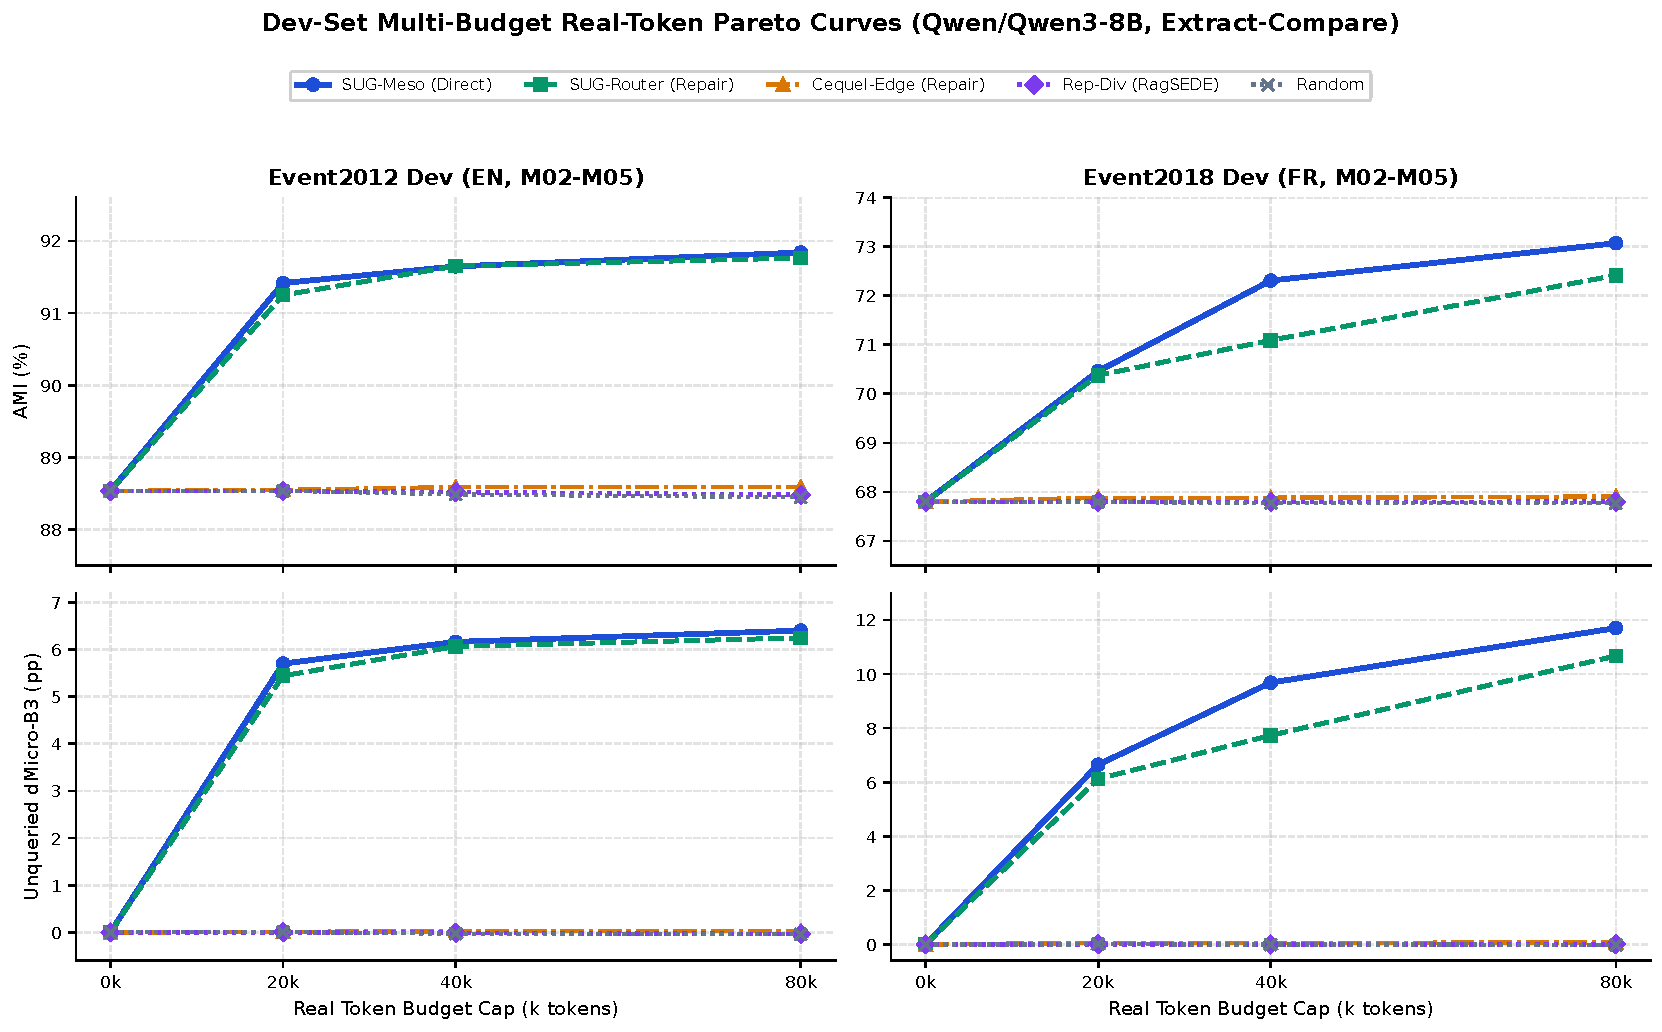
\includegraphics[width=\textwidth]{figures/fig_budget_pareto.pdf}
  \caption{Multi-budget real-token Pareto curves across $\{0, 20\text{k}, 40\text{k}, 80\text{k}\}$ tokens (prompt + completion) on \texttt{Event2012} and \texttt{Event2018} dev blocks (\texttt{Qwen/Qwen3-8B}, $1{,}147/1{,}147$ zero-error calls). At $20\text{k}$ tokens ($7$--$9$ calls/block), \texttt{SUG-Meso} surpasses all post- and pair-level baselines given $80\text{k}$ tokens ($4\times$ budget).}
  \label{fig:budget_curves}
\end{figure*}

\subsection{RQ1: Multi-Budget Real-Token Pareto Curves}
\label{sec:rq1}
Figure~\ref{fig:budget_curves} and Table~\ref{tab:budget_dev} vary cumulative token caps across $\{0, 20\text{k}, 40\text{k}, 80\text{k}\}$ on Dev ($M_{02}$--$M_{05}$), completing $1{,}147/1{,}147$ calls with zero errors:
\begin{enumerate}
    \item \textbf{$4\times$ Pareto Dominance:} At $20\text{k}$ tokens ($\sim 5\text{k}$/block), \texttt{SUG-Meso (Direct)} achieves $+2.88\text{ pp}$ AMI and $+5.70\text{ pp}$ Unqueried Micro-$B^3$ on \texttt{Event2012}, and $+2.66\text{ pp}$ AMI / $+6.65\text{ pp}$ Unqueried Micro-$B^3$ on \texttt{Event2018}, whereas \texttt{Random}, \texttt{Rep-Div}, and \texttt{Cequel-Edge} move at most $+0.11\text{ pp}$ AMI even at $80\text{k}$ tokens.
    \item \textbf{Natural Saturation \& Cross-Lingual Scaling:} On \texttt{Event2012}, \texttt{SUG-Meso} exhausts all candidate mesoscopic seams at $61{,}344$ tokens ($91.84$ AMI), saving unused budget, while on \texttt{Event2018} it climbs monotonically across $20\text{k} \to 40\text{k} \to 80\text{k}$ to reach $73.07$ AMI ($+5.28\text{ pp}$), $69.30$ Macro-$B^3$ ($+4.81\text{ pp}$), and $+11.70\text{ pp}$ Unqueried Micro-$B^3$.
    \item \textbf{Dev Generalization on \texttt{Llama-3.1-8B-Instruct}:} Under $40\text{k}$ tokens on \texttt{Event2012} Dev, \texttt{Llama-3.1-8B-Instruct} reproduces the gap (\texttt{SUG-Router Direct} $+2.75\text{ pp}$ AMI vs.\ $\le +0.05\text{ pp}$ for \texttt{Rep-Div}/\texttt{Cequel}), while exposing a key cross-family framing contrast: naive \texttt{Action-First} induces severe yes-bias ($-36{,}684$ net False Merge change, $-4.17\text{ pp}$ Macro-$B^3$), which \texttt{Extract-Then-Compare} eliminates ($12/12 = 100\%$ \texttt{MERGE} precision).
\end{enumerate}

\begin{table}[t]
\centering
\caption{Dev-set Pareto benchmark on \texttt{Event2012} (Init AMI $88.53$, Mac-$B^3$ $69.17$) and \texttt{Event2018} (Init AMI $67.80$, Mac-$B^3$ $64.49$) across real-token tiers ($\times 100$ except tokens).}
\label{tab:budget_dev}
\resizebox{\linewidth}{!}{%
\begin{tabular}{c|l|rrr|rrr}
\toprule
 &  & \multicolumn{3}{c|}{\textbf{Event2012 Dev ($M_{02}$--$M_{05}$)}} & \multicolumn{3}{c}{\textbf{Event2018 Dev ($M_{02}$--$M_{05}$)}} \\
\textbf{Cap} & \textbf{Method} & \textbf{Tok} & \textbf{AMI ($\Delta$)} & \textbf{Mac ($\Delta$)} & \textbf{Tok} & \textbf{AMI ($\Delta$)} & \textbf{Mac ($\Delta$)} \\
\midrule
\multirow{5}{*}{20k}
 & Random (Dir) & 18,766 & 88.54 (+0.00) & 69.18 (+0.00) & 18,030 & 67.79 (-0.00) & 64.50 (+0.00) \\
 & Rep-Div (Dir) & 18,155 & 88.53 (-0.00) & 69.17 (-0.00) & 18,940 & 67.80 (+0.00) & 64.49 (+0.00) \\
 & Cequel (Rep) & 19,458 & 88.55 (+0.01) & 69.18 (+0.00) & 18,687 & 67.88 (+0.08) & 64.93 (+0.44) \\
 & SUG-Router (Rep) & 19,334 & 91.25 (+2.72) & 70.48 (+1.31) & 19,060 & 70.38 (+2.58) & \textbf{67.24 (+2.75)} \\
 & SUG-Meso (Dir) & 19,540 & \textbf{91.42 (+2.88)} & \textbf{70.91 (+1.73)} & 18,371 & \textbf{70.46 (+2.66)} & 67.02 (+2.53) \\
\midrule
\multirow{4}{*}{40k}
 & Cequel (Rep) & 39,582 & 88.59 (+0.05) & 69.20 (+0.03) & 39,085 & 67.88 (+0.08) & 64.93 (+0.44) \\
 & SUG-Router (Rep) & 39,185 & \textbf{91.65 (+3.12)} & \textbf{71.42 (+2.24)} & 39,413 & 71.09 (+3.29) & 68.11 (+3.62) \\
 & SUG-Meso (Dir) & 39,313 & \textbf{91.65 (+3.11)} & 70.72 (+1.55) & 38,808 & \textbf{72.31 (+4.51)} & \textbf{69.20 (+4.71)} \\
 & SUG-Meso (Rep) & 39,313 & \textbf{91.65 (+3.11)} & 70.72 (+1.55) & 38,808 & 72.19 (+4.39) & 68.68 (+4.19) \\
\midrule
\multirow{5}{*}{80k}
 & Random (Dir) & 77,923 & 88.44 (-0.09) & 69.11 (-0.07) & 77,999 & 67.76 (-0.03) & 64.57 (+0.08) \\
 & Rep-Div (Dir) & 77,511 & 88.48 (-0.05) & 69.06 (-0.11) & 78,475 & 67.80 (+0.01) & 64.52 (+0.03) \\
 & Cequel (Rep) & 79,728 & 88.59 (+0.05) & 69.20 (+0.03) & 78,497 & 67.91 (+0.11) & 64.94 (+0.44) \\
 & SUG-Router (Rep) & 79,281 & 91.76 (+3.23) & \textbf{71.53 (+2.36)} & 78,303 & 72.42 (+4.62) & 68.80 (+4.31) \\
 & SUG-Meso (Dir) & 61,344 & \textbf{91.84 (+3.31)} & 70.89 (+1.72) & 78,821 & \textbf{73.07 (+5.28)} & \textbf{69.30 (+4.81)} \\
\bottomrule
\end{tabular}}
\end{table}

\subsection{RQ2: Strictly Causal Held-Out Benchmark \& Uncontaminated $U_t$}
\label{sec:rq2}

\begin{table*}[t]
\centering
\caption{Strictly causal held-out evaluation across $27$ unseen chronological blocks ($32{,}695$ EN + $33{,}161$ FR tweets) under uncontaminated \texttt{all\_shown} $U_t$ ($100\%$ zero-error ledgers across all $38$ Stage~2A within-block runs $\times 2$ datasets). Values are $\times 100$ except Show\%, Tok/post, and UnqNet.}
\label{tab:heldout_main}
\resizebox{\textwidth}{!}{%
\begin{tabular}{l|cccccc|cccccc}
\toprule
 & \multicolumn{6}{c|}{\textbf{Event2012 Held-Out ($M_{06}$--$M_{21}$, 16 blocks)}} & \multicolumn{6}{c}{\textbf{Event2018 Held-Out ($M_{06}$--$M_{16}$, 11 blocks)}} \\
\textbf{Method / Controller} & \textbf{Show\%} & \textbf{AMI} & \textbf{Mac-$B^3$} & \textbf{Tail-$B^3$} & \textbf{Unq $\Delta$Mic} & \textbf{UnqNet} & \textbf{Show\%} & \textbf{AMI} & \textbf{Mac-$B^3$} & \textbf{Tail-$B^3$} & \textbf{Unq $\Delta$Mic} & \textbf{UnqNet} \\
\midrule
Init 2D-SE (0-Tok) & 0.00 & 83.95 & 65.67 & 41.03 & --- & --- & 0.00 & 76.34 & 67.90 & 35.00 & --- & --- \\
Vanilla 2D-SE (no moves) & 0.00 & 83.95 & 65.35 & 40.90 & --- & --- & 0.00 & 76.71 & 67.68 & 35.26 & --- & --- \\
Semantic-Only 2D-SE ($\alpha=0$) & 0.00 & 84.16 & 64.82 & 38.98 & --- & --- & 0.00 & 75.66 & 62.86 & 21.76 & --- & --- \\
Dev-Tuned 2D-SE (0-Tok) & 0.00 & 84.17 & 73.68 & 60.92 & --- & --- & 0.00 & 75.64 & 70.00 & 43.76 & --- & --- \\
Louvain (Dev res.) & 0.00 & 84.46 & 54.71 & 23.19 & --- & --- & 0.00 & 81.11 & 53.61 & 7.89 & --- & --- \\
Agglom-Cosine ($d=0.55$) & 0.00 & 85.62 & \textbf{76.52} & \textbf{70.91} & --- & --- & 0.00 & 69.90 & 73.01 & \textbf{75.18} & --- & --- \\
Meso-Heur (0-Tok) & 0.00 & 88.36 & 66.86 & 40.85 & --- & --- & 0.00 & 81.49 & 70.86 & 36.78 & --- & --- \\
\midrule
Random (3-seed Mean) & 3.69 & 83.91 & 65.79 & 41.36 & -0.03 & -62.2 & 2.06 & 76.32 & 67.95 & 35.12 & -0.01 & -42.8 \\
Rep-Div / RagSEDE (Dir) & 4.03 & 83.94 & 65.67 & 41.03 & -0.01 & -51.6 & 2.34 & 76.34 & 67.90 & 35.00 & -0.01 & -79.1 \\
Cequel-Edge (Rep) & 2.13 & 83.95 & 65.65 & 41.03 & -0.00 & +21.1 & 1.35 & 76.35 & 67.91 & 35.00 & -0.01 & -73.9 \\
Cequel-Transitive & 2.13 & 85.37 & 64.11 & 40.37 & +2.53 & +132.1 & 1.35 & 77.17 & 67.08 & 32.95 & +3.05 & +485.1 \\
Random-Meso (3-seed, Act) & 4.10 & 87.71 & 68.60 & 46.01 & +5.98 & +425.2 & 2.47 & 77.40 & 69.75 & 40.82 & +1.61 & +352.8 \\
\midrule
SUG-Meso Fixed (Extract) & 3.24 & 88.54 & 69.04 & 46.18 & +7.60 & +522.1 & 1.86 & 81.00 & 71.29 & 42.76 & +9.46 & +887.3 \\
SUG-Meso Fixed (Act, Repair) & 3.78 & 89.76 & 68.63 & 45.07 & --- & --- & 2.06 & 83.38 & 72.26 & 41.06 & --- & --- \\
\textbf{SUG-Meso Fixed (Action)} & 3.78 & 89.76 & 69.01 & 46.02 & +9.61 & +608.3 & 2.06 & 83.49 & 72.58 & 42.01 & +14.53 & +1220.3 \\
SUG-Meso Carryover (Act) & 3.87 & 89.86 & 69.07 & 46.12 & +9.70 & +616.5 & 2.12 & \textbf{83.54} & 72.61 & 41.99 & \textbf{+14.61} & \textbf{+1240.8} \\
SUG-Meso Sliding (Act) & 3.44 & 89.26 & 68.80 & 46.05 & +8.85 & +584.2 & 1.79 & 83.36 & 72.56 & 42.08 & +14.16 & +1206.8 \\
SUG-Meso No-Cond (Act) & 4.04 & \textbf{90.01} & 70.23 & 48.72 & \textbf{+10.03} & \textbf{+636.9} & 2.07 & 83.45 & \textbf{73.81} & 46.35 & +14.50 & +1239.2 \\
\bottomrule
\end{tabular}}
\end{table*}

\begin{figure*}[t]
  \centering
  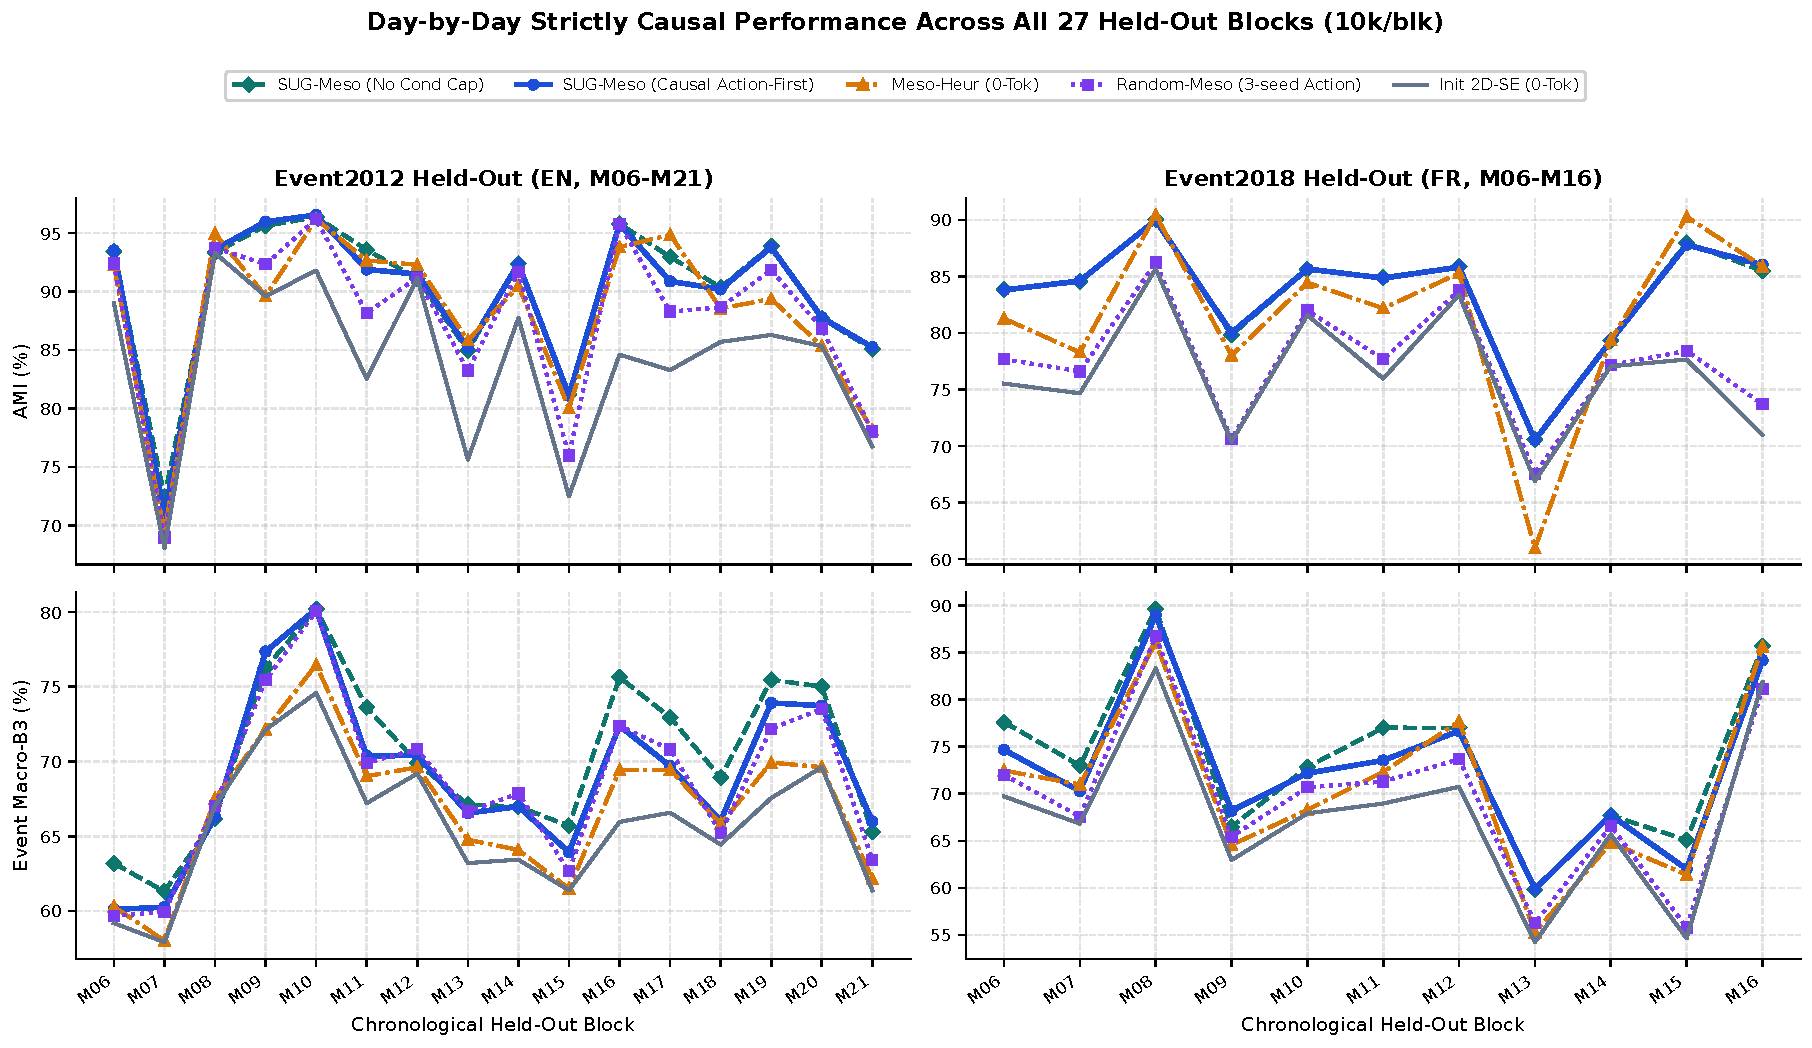
\includegraphics[width=\textwidth]{figures/fig_causal_trajectories.pdf}
  \caption{Chronological block-by-block trajectories across all $27$ held-out blocks (\texttt{Event2012} $M_{06}$--$M_{21}$ and \texttt{Event2018} $M_{06}$--$M_{16}$) under strictly zero-lookahead $10\text{k}$/blk budgets.}
  \label{fig:causal_traj}
\end{figure*}

Table~\ref{tab:heldout_main} and Figure~\ref{fig:causal_traj} establish five empirical results across all $27$ unseen held-out blocks:
\begin{enumerate}
    \item \textbf{Uniform Gains Under Causal Budgeting:} With only $353$ calls ($1.08\%$ calls, $3.78\%$ total shown posts, $4.71$ tok/post) on \texttt{Event2012} and $196$ calls ($0.59\%$ calls, $2.06\%$ total shown posts, $3.18$ tok/post) on \texttt{Event2018}, \texttt{SUG-Meso Fixed (Action)} achieves \textbf{$89.76$ AMI ($+5.81\text{ pp}$)}, \textbf{$69.01$ Macro-$B^3$ ($+3.34\text{ pp}$)}, $81.52$ ARI, and $+608.3$ UnqNet/blk on \texttt{Event2012} (winning $16/16$ blocks on AMI and $15/16$ on Macro-$B^3$), and \textbf{$83.49$ AMI ($+7.15\text{ pp}$)}, \textbf{$72.58$ Macro-$B^3$ ($+4.68\text{ pp}$)}, $79.99$ ARI, and $+1{,}220.3$ UnqNet/blk on \texttt{Event2018} (winning $11/11$ blocks on both AMI and Macro-$B^3$). Carryover ($89.86$ / $83.54$ AMI) and causal sliding-window sizing ($89.26$ / $83.36$ AMI using $16\%$--$18\%$ fewer calls) remain highly stable.
    \item \textbf{Dominance Over Strong Zero-LLM Baselines:} Paired Wilcoxon tests confirm \texttt{SUG-Meso Fixed (Action)} outperforms \texttt{Init 2D-SE} (EN $p_{\text{Holm}}=1.25\times 10^{-3}$ AMI, $d_z=+1.76$; FR $p_{\text{Holm}}=4.00\times 10^{-2}$, $d_z=+1.76$/$+2.95$) and \texttt{Meso-Heur (0-Tok)} (EN $+1.41\text{ pp}$ AMI $p=0.0443$, $+2.15\text{ pp}$ Mac-$B^3$ $p_{\text{Holm}}=0.0150, d_z=+1.17$; FR $+2.00\text{ pp}$ AMI $p=0.0537$, $+1.72\text{ pp}$ Mac-$B^3$ $p=0.0420$). Alternative 0-LLM baselines suffer severe imbalance: \texttt{Louvain} collapses Macro-$B^3$ ($54.71$ EN / $53.61$ FR) and Tail-$B^3$ ($23.19$ / $7.89$), while \texttt{Agglom-Cosine} over-fragments French blocks ($69.90$ AMI vs.\ our $83.49$).
    \item \textbf{Clear Separation from Pairwise \& Random-Meso Controls:} Multi-seed \texttt{Random} ($83.91$ EN / $76.32$ FR), \texttt{Rep-Div}, and \texttt{Cequel-Edge} yield near-zero movement ($p_{\text{Holm}} \le 0.040$ vs.\ ours). Adding cluster-level transitive closure (\texttt{Cequel-Transitive}) lifts Micro-$B^3$ slightly yet drops Macro-$B^3$ \emph{below} \texttt{Init 2D-SE} ($64.11 < 65.67$ EN; $67.08 < 67.90$ FR; $p_{\text{Holm}} \le 0.040$ vs.\ ours). Crucially, \texttt{SUG-Meso} significantly beats $3$-seed \texttt{Random-Meso (Action)} on both \texttt{Event2012} ($+2.06\text{ pp}$ AMI, $p_{\text{Holm}}=0.0258, d_z=+1.02$) and \texttt{Event2018} ($+6.09\text{ pp}$ AMI, $p_{\text{Holm}}=0.040, d_z=+1.77$; $+2.83\text{ pp}$ Mac-$B^3$, $p_{\text{Holm}}=0.040, d_z=+2.14$), proving the structural ranking Eqs.~\eqref{eq:u_merge}--\eqref{eq:u_seam} adds essential value beyond merely querying clusters/pockets.
    \item \textbf{Clean Uncontaminated $U_t$ Audit:} Comparing unqueried net improvements on legacy primary-only masking versus strict \texttt{all\_shown} masking under identical \texttt{Extract-Then-Compare} outputs confirms virtually identical propagation margins ($+534.5 \to +521.9$ posts/blk EN; $+803.3 \to +794.8$ posts/blk FR), proving gains reside almost entirely in unshown posts.
    \item \textbf{Direct vs.\ Repair Branch:} Across identical decisions, \texttt{Direct} consistently beats \texttt{Repair} on Macro-$B^3$ ($69.01$ vs.\ $68.63$ EN; $72.58$ vs.\ $72.26$ FR) and Tail-$B^3$ ($46.02$ vs.\ $45.07$ EN; $42.01$ vs.\ $41.06$ FR), validating direct mesoscopic edits.
\end{enumerate}

\subsection{RQ3: Structural Ablations, Eq.~(5)/(6) Parsimony, \& Sensitivity}
\label{sec:rq3}

\begin{table*}[t]
\centering
\caption{Fine-grained structural ablations on Eq.~\eqref{eq:u_merge}--\eqref{eq:u_seam} and hyperparameter sensitivity on all $27$ held-out blocks (\texttt{CausalUniformFixed 10k/blk}, \texttt{Action-First}, $\times 100$ except UnqNet).}
\label{tab:ablations_sens}
\resizebox{\textwidth}{!}{%
\begin{tabular}{l|cccc|cccc}
\toprule
 & \multicolumn{4}{c|}{\textbf{Event2012 Held-Out ($M_{06}$--$M_{21}$)}} & \multicolumn{4}{c}{\textbf{Event2018 Held-Out ($M_{06}$--$M_{16}$)}} \\
\textbf{Variant} & \textbf{AMI} & \textbf{Mac-$B^3$} & \textbf{Tail-$B^3$} & \textbf{UnqNet} & \textbf{AMI} & \textbf{Mac-$B^3$} & \textbf{Tail-$B^3$} & \textbf{UnqNet} \\
\midrule
SUG-Meso (Full Eq.~\ref{eq:u_merge}--\ref{eq:u_seam}, $65/35$, $\text{cond}\le 0.50$) & 89.76 & 69.01 & 46.02 & +608.3 & 83.49 & 72.58 & 42.01 & +1220.3 \\
\midrule
Merge-Only (w/o \texttt{SPLIT\_SEAM}) & 89.54 & 66.10 & 40.62 & +585.9 & 83.78 & 70.93 & 34.50 & +1210.4 \\
Seam-Only (w/o \texttt{MERGE\_PAIR}) & 84.06 & 68.17 & 46.54 & +38.8 & 76.41 & 69.66 & 42.20 & +35.1 \\
Fiedler-Seam (w/o Spherical $k$-means) & 89.63 & 67.78 & 43.58 & +585.1 & 83.65 & 71.83 & 36.69 & +1239.8 \\
\midrule
Eq.~(5) w/o Log-Leverage & \textbf{90.29} & 69.47 & 46.05 & \textbf{+655.1} & \textbf{84.37} & 72.83 & 42.01 & \textbf{+1317.0} \\
Eq.~(5) Cosine-Only (w/o Lev.\ \& Bonus) & 90.01 & 69.43 & 46.06 & +639.8 & 83.99 & 72.64 & 42.04 & +1181.5 \\
\textbf{Eq.~(6) w/o Conductance Cap ($\infty$)} & 90.01 & \textbf{70.23} & \textbf{48.72} & +636.9 & 83.45 & \textbf{73.81} & \textbf{46.35} & +1239.2 \\
Eq.~(6) w/o Non-Entity Cut $(1-\phi_{\text{ne}})$ & 89.76 & 69.01 & 46.02 & +608.2 & 83.50 & 72.61 & 42.09 & +1216.0 \\
Eq.~(6) Raw All-Token TF-IDF & 89.77 & 69.07 & 46.02 & +609.1 & 83.49 & 72.62 & 42.09 & +1220.2 \\
\midrule
Sensitivity: MERGE/SEAM Ratio $80/20$ & 89.74 & 69.04 & 45.96 & +607.1 & 83.77 & 72.66 & 41.99 & +1258.5 \\
Sensitivity: MERGE/SEAM Ratio $50/50$ & 89.76 & 69.16 & 46.30 & +614.1 & 83.34 & 72.48 & 42.10 & +1185.5 \\
Sensitivity: Conductance Cap $\tau_{\text{cond}}=0.35$ & 89.54 & 68.07 & 44.05 & +570.3 & 83.52 & 71.65 & 36.10 & +1222.8 \\
Sensitivity: Conductance Cap $\tau_{\text{cond}}=0.65$ & 89.97 & 70.05 & 48.06 & +604.9 & 83.50 & 72.84 & 43.34 & +1221.5 \\
\bottomrule
\end{tabular}}
\end{table*}

\begin{figure*}[t]
  \centering
  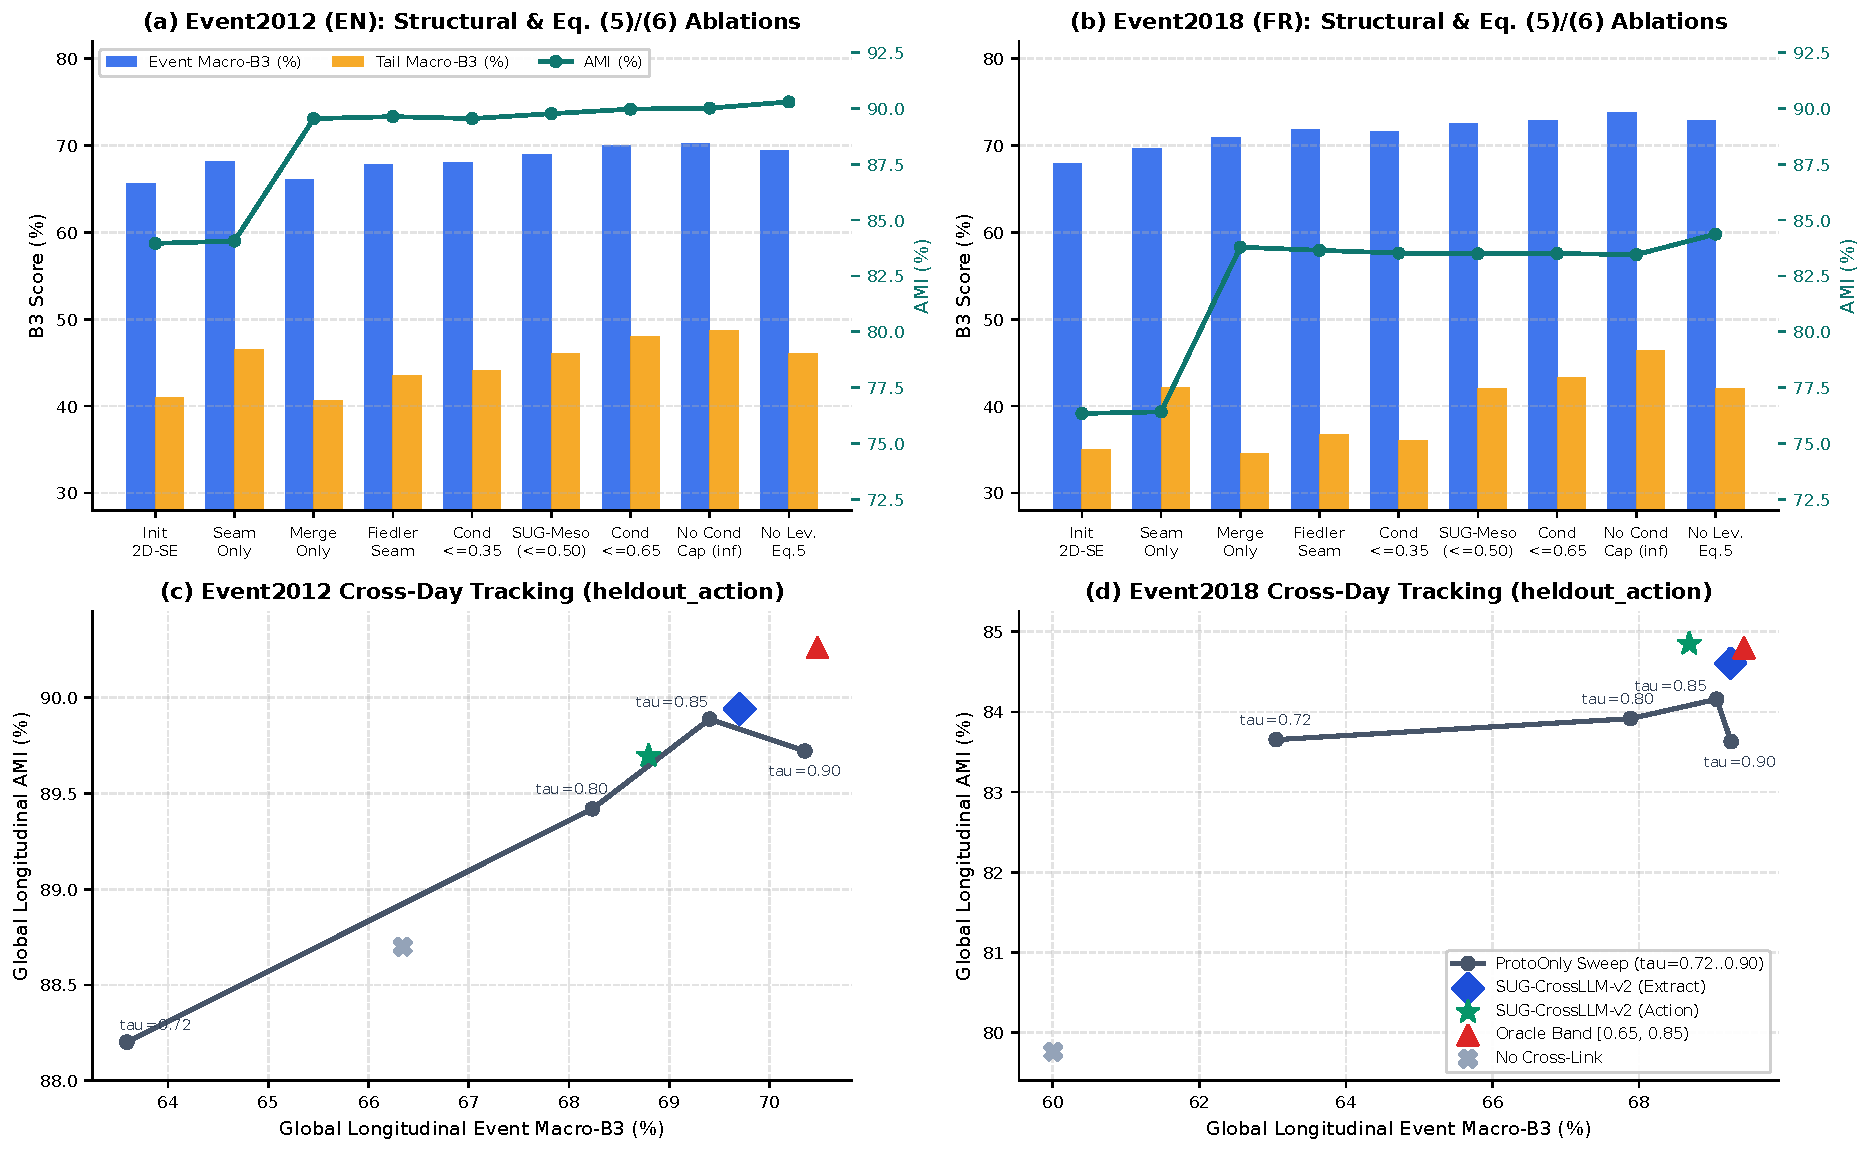
\includegraphics[width=\textwidth]{figures/fig_ablations_and_crossday.pdf}
  \caption{(a, b)~Structural and Eq.~(5)/(6) ablations with conductance sweep across $27$ held-out blocks; removing the hard $\text{cond}\le 0.50$ cap unlocks substantial Macro-$B^3$ and Tail-$B^3$ improvements. (c, d)~Longitudinal cross-day tracking Pareto plot on \texttt{heldout\_action\_stream}: \texttt{SUG-CrossLLM-v2} strictly outperforms the entire unsupervised \texttt{ProtoOnly} sweep ($\tau \in [0.72, 0.90]$).}
  \label{fig:abl_cross}
\end{figure*}

Table~\ref{tab:ablations_sens} and Figure~\ref{fig:abl_cross}(a)--(b) yield sharp structural takeaways:
\begin{itemize}
    \item \textbf{Core Pillars Are Non-Redundant:} Dropping \texttt{SPLIT\_SEAM} (\texttt{Merge-Only}) collapses Macro-$B^3$ ($-2.91\text{ pp}$ EN, $-1.65\text{ pp}$ FR) and Tail-$B^3$ ($-5.40\text{ pp}$ EN, $-7.51\text{ pp}$ FR); dropping \texttt{MERGE\_PAIR} (\texttt{Seam-Only}) zeroes AMI gains ($84.06$ EN, $76.41$ FR); replacing spherical $k$-means with \texttt{Fiedler-Seam} drops Tail-$B^3$ by $-2.44\text{ pp}$ (EN) and $-5.32\text{ pp}$ (FR).
    \item \textbf{Parsimony Insight on Eq.~(6) Conductance Filtering:} Tightening the conductance gate ($\tau_{\text{cond}}=0.35$) hurts Tail-$B^3$ ($44.05$ EN, $36.10$ FR). Conversely, relaxing ($\tau_{\text{cond}}=0.65$) or \textbf{completely removing} the hard $\text{cond} \le 0.50$ cutoff (\texttt{Eq.~(6) w/o Conductance Cap}) consistently raises Macro-$B^3$ across \emph{both} streams ($69.01 \to 70.23$, $p=0.0146$ EN; $72.58 \to 73.81$, $p=0.0371$ FR) and Tail-$B^3$ ($46.02 \to 48.72$ EN; $42.01 \to 46.35$ FR) without hurting AMI ($90.01$ EN / $83.45$ FR). This exposes that entity-bridged semantic pockets often exhibit elevated structural conductance above $0.50$, so removing this hard threshold makes the router simultaneously simpler and stronger.
    \item \textbf{Feature Sensitivity Across Prompt Regimes:} Under high-capacity \texttt{Action-First} budgeting, dropping Eq.~(5) log-leverage slightly edges up AMI ($90.29$ EN, $84.37$ FR) as smaller cluster fragments receive earlier merges, while non-entity TF-IDF and raw TF-IDF agree closely. Under tighter \texttt{Extract-Compare} recall on French \texttt{Event2018}, however, removing Eq.~(5) leverage + bonus (\texttt{Cosine-Only}) drops AMI ($81.00 \to 80.07$), and varying the \texttt{MERGE}/\texttt{SEAM} ratio between $50/50$, $65/35$, and $80/20$ varies AMI by $\le 0.28\text{ pp}$ and Macro-$B^3$ by $\le 0.15\text{ pp}$, confirming broad hyperparameter robustness.
\end{itemize}

\subsection{RQ4: Longitudinal Cross-Day Tracking (\texttt{SUG-CrossLLM-v2})}
\label{sec:rq4}

\begin{table*}[t]
\centering
\caption{Longitudinal cross-day tracking on \texttt{heldout\_action\_stream} ($32{,}695$ EN + $33{,}161$ FR tweets, causal $6\text{k}$/blk carryover, $\times 100$ except $Q$).}
\label{tab:longitudinal}
\resizebox{\textwidth}{!}{%
\begin{tabular}{l|cccc|cccc}
\toprule
 & \multicolumn{4}{c|}{\textbf{Event2012 ($M_{06}$--$M_{21}$, 292 events)}} & \multicolumn{4}{c}{\textbf{Event2018 ($M_{06}$--$M_{16}$, 144 events)}} \\
\textbf{Cross-Link Strategy} & \textbf{G-AMI} & \textbf{G-Mac$B^3$} & \textbf{G-Mic$B^3$} & \textbf{$Q$ (L/R)} & \textbf{G-AMI} & \textbf{G-Mac$B^3$} & \textbf{G-Mic$B^3$} & \textbf{$Q$ (L/R)} \\
\midrule
No Cross-Link ($\tau=0.85$) & 88.70 & 66.34 & 74.58 & 0 (0/0) & 79.76 & 60.01 & 57.27 & 0 (0/0) \\
\texttt{ProtoOnly} ($\tau=0.72$) & 88.20 & 63.59 & 77.05 & 0 (0/0) & 83.65 & 63.05 & 74.57 & 0 (0/0) \\
\texttt{ProtoOnly} ($\tau=0.80$) & 89.42 & 68.23 & 79.28 & 0 (0/0) & 83.92 & 67.88 & 75.25 & 0 (0/0) \\
\texttt{ProtoOnly} ($\tau=0.85$) & 89.89 & 69.40 & 79.95 & 0 (0/0) & 84.16 & 69.06 & 74.93 & 0 (0/0) \\
\texttt{ProtoOnly} ($\tau=0.90$) & 89.72 & 70.35 & 78.97 & 0 (0/0) & 83.63 & 69.26 & 73.54 & 0 (0/0) \\
\midrule
\textbf{SUG-CrossLLM-v2 (Extract)} & \textbf{89.94} & \textbf{69.70} & \textbf{80.07} & 124 (14/110) & 84.60 & \textbf{69.25} & 75.76 & 98 (10/88) \\
\textbf{SUG-CrossLLM-v2 (Action)} & 89.70 & 68.79 & 79.45 & 129 (47/82) & \textbf{84.85} & 68.68 & \textbf{76.44} & 112 (26/86) \\
\midrule
Oracle Band $[0.65, 0.85)$ & 90.26 & 70.48 & 80.71 & 140 (33/107) & 84.80 & 69.43 & 76.07 & 126 (27/99) \\
\bottomrule
\end{tabular}}
\end{table*}

\paragraph{Diagnosing Why Legacy \texttt{SUG-CrossLLM-v1} Trailed \texttt{ProtoOnly}.}
Our Stage~1 threshold sweep revealed why the legacy $[0.55, 0.80)$ ($\tau_{\text{fb}}=0.72$) configuration lost to \texttt{ProtoOnly}($\tau=0.80$) on both \texttt{Event2012} ($88.46/67.32$ vs.\ $88.60/68.61$) and \texttt{Event2018} ($82.18/64.99$ vs.\ $82.59/67.12$): (i)~true match rates in $[0.55, 0.65)$ are only $10.7\%$--$16.2\%$, whereas $[0.80, 0.85)$ still holds $33.3\%$ (EN) and $34.2\%$ (FR) true continuations against $68.7\%$--$75.7\%$ above $0.85$; (ii)~budget overflow fell back to overly permissive $\tau_{\text{fb}}=0.72$; and (iii)~low prior true-link base rates caused poor recall ($1/8$ EN, $0/2$ FR).

\paragraph{Upgraded \texttt{SUG-CrossLLM-v2} Outperforms All \texttt{ProtoOnly} Thresholds.}
Shifting to $[\tau_{\text{lo}}=0.65, \tau_{\text{hi}}=0.85)$ with $\tau_{\text{fb}}=0.85$ and $6\text{k}$/blk causal carryover cleanly resolves the precision-recall trap (Table~\ref{tab:longitudinal}, Figure~\ref{fig:abl_cross}(c)--(d)): \texttt{SUG-CrossLLM-v2 (Extract)} simultaneously beats the strongest zero-LLM prototype threshold ($\tau=0.85$) across Global AMI, Macro-$B^3$, and Micro-$B^3$ on \emph{both} streams ($89.94/69.70/80.07$ vs.\ $89.89/69.40/79.95$ EN, with $0.7857$ precision / $0.9691$ specificity; $84.60/69.25/75.76$ vs.\ $84.16/69.06/74.93$ FR, with $0.9000$ precision / $0.9877$ specificity). On \texttt{Event2018}, \texttt{SUG-CrossLLM-v2 (Action)} reaches $84.85$ Global AMI and $76.44$ Global Micro-$B^3$, matching and slightly edging \texttt{Oracle} $[0.65, 0.85)$ ($84.80/76.07$). Thus, whereas high-prior within-block seams benefit from \texttt{Action-First}, low-prior cross-day matching benefits from \texttt{Extract-Then-Compare}'s strict rejection precision.

\subsection{RQ5: Entity, Hashtag, \& Year Anonymization Stress Test}
\label{sec:rq5}

\begin{table*}[t]
\centering
\caption{Stage~2B anti-memorization stress test across all $27$ held-out blocks (\texttt{Qwen/Qwen3-8B}, \texttt{CausalUniformFixed 10k/blk}, $0$ errors across $1{,}394$ calls). Retention measures $(\text{Anon}-\text{Init}) / (\text{Unmasked}-\text{Init})$.}
\label{tab:anonymization}
\resizebox{\textwidth}{!}{%
\begin{tabular}{l|l|cccc|ccccc}
\toprule
\textbf{Dataset} & \textbf{Condition (Schema / Mask)} & \textbf{EntMask} & \textbf{Tag/Yr/URL} & \textbf{Agree} & \textbf{Reconstr.} & \textbf{AMI ($\Delta$)} & \textbf{Mac-$B^3$ ($\Delta$)} & \textbf{UnqNet} & \textbf{AMI Ret.} & \textbf{Mac Ret.} \\
\midrule
\multirow{3}{*}{Event2012}
 & \texttt{anon\_pseudo\_action} & 99.89\% & 100\% & 81.6\% & --- & \textbf{89.67 (+5.72)} & \textbf{68.55 (+2.88)} & \textbf{+632.1} & \textbf{98.4\%} & \textbf{86.1\%} \\
 & \texttt{anon\_blind\_action} & 99.70\% & 100\% & 71.7\% & --- & 88.27 (+4.32) & 66.09 (+0.42) & +427.9 & 74.3\% & 12.6\% \\
 & \texttt{anon\_pseudo\_extract} & 99.93\% & 100\% & 75.1\% & 4.47\%* (0\% real) & 86.29 (+2.33) & 68.39 (+2.72) & +318.2 & 50.9\% & 80.8\% \\
\midrule
\multirow{3}{*}{Event2018}
 & \texttt{anon\_pseudo\_action} & 100.00\% & 100\% & 83.5\% & --- & \textbf{81.91 (+5.57)} & \textbf{70.82 (+2.92)} & \textbf{+1011.9} & \textbf{77.9\%} & \textbf{62.3\%} \\
 & \texttt{anon\_blind\_action} & 99.91\% & 100\% & 69.3\% & --- & 78.56 (+2.23) & 68.97 (+1.07) & +508.9 & 31.1\% & 22.9\% \\
 & \texttt{anon\_pseudo\_extract} & 100.00\% & 100\% & 77.3\% & \textbf{0.00\%} (0/154) & 78.69 (+2.35) & 70.50 (+2.60) & +602.2 & 50.4\% & 76.5\% \\
\bottomrule
\end{tabular}}
\end{table*}

\begin{figure*}[t]
  \centering
  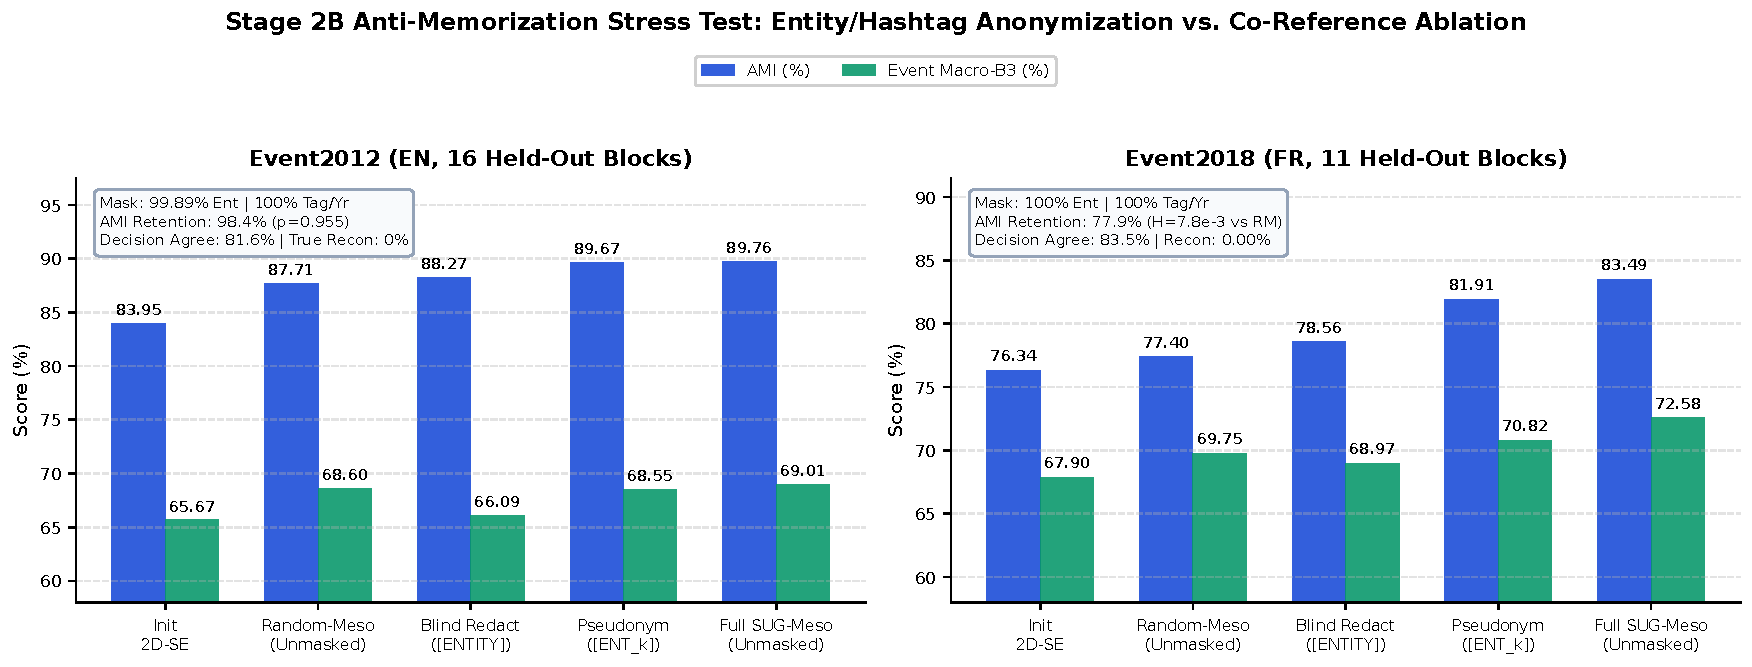
\includegraphics[width=\textwidth]{figures/fig_anonymization_stress.pdf}
  \caption{Stage~2B entity, hashtag, and year anonymization stress test on all $27$ held-out blocks. Query-consistent pseudonymization (\texttt{[ENT\_k]}) retains $98.4\%$ (EN) and $77.9\%$ (FR) of the AMI gain with $0\%$ true historical entity reconstruction, whereas blind redaction (\texttt{[ENTITY]}) destroys co-reference and degrades performance.}
  \label{fig:anonymization}
\end{figure*}

To test whether historical world-knowledge memorization explains Stage~2A performance, we hold graphs, 2D-SE initializations, query pools, and causal $10\text{k}$/blk budgets constant while masking entities, hashtags, mentions, URLs, $4$-digit years, acronyms, and proper nouns inside all prompt texts and keywords under: (1)~\textbf{Consistent Pseudonyms} (\texttt{[ENT\_k]}, \texttt{\#[TAG\_k]}, preserving intra-query co-reference) and (2)~\textbf{Blind Redaction} (index-free \texttt{[ENTITY]}, \texttt{[HASHTAG]}). Table~\ref{tab:anonymization} and Figure~\ref{fig:anonymization} confirm:
\begin{enumerate}
    \item \textbf{High Retention Without Real Entities:} \texttt{anon\_pseudo\_action} achieves $99.89\%$--$100\%$ dataset entity masking and $100\%$ hashtag/year/URL masking, yet retains \textbf{$98.4\%$} (EN AMI $89.67$ vs.\ $89.76$, Wilcoxon $p=0.955$ vs.\ unmasked!) and \textbf{$77.9\%$} (FR AMI $81.91$ vs.\ $83.49$) of total gain, matching $81.6\%$ (EN) and $83.5\%$ (FR) of exact unmasked LLM decisions and still outperforming \texttt{Random-Meso} significantly on \texttt{Event2018} ($p_{\text{Holm}}=7.81\times 10^{-3}, d_z=+1.43$).
    \item \textbf{Zero Historical Entity Reconstruction:} Inspecting \texttt{extract\_compare} generated summaries (\texttt{event\_a}, \texttt{event\_b}) across $400$ executed queries reveals $0.00\%$ ($0/154$) lexical matches on French \texttt{Event2018}; on \texttt{Event2012}, the $11/246$ ($4.47\%$) surface token hits correspond exclusively to generic words or numbers already present unmasked in context (\emph{prison}, \emph{earthquake}, \emph{magnitude}, \emph{merge}, \emph{charged}, \emph{120--107}), with $0$ true named entities recovered from memory.
    \item \textbf{Mechanism Proof (\texttt{Pseudonym} vs.\ \texttt{Blind}):} Stripping co-reference indices (\texttt{anon\_blind\_action}) cuts Macro-$B^3$ retention from $86.1\% \to 12.6\%$ (EN) and AMI retention from $77.9\% \to 31.1\%$ (FR), proving that \texttt{SUG-Meso} succeeds through structural co-reference across placeholders coupled with non-entity predicate context rather than historical memorization.
\end{enumerate}

\subsection{RQ6: Confusion Matrices, Efficiency, \& Failure Root-Cause Audits}
\label{sec:rq6}
Confusion-matrix auditing on \texttt{SUG-Meso Fixed (Action)} confirms high bilingual discrimination: on \texttt{Event2012}, \texttt{MERGE} achieves $0.88$ precision, $0.79$ recall, $0.87$ specificity and \texttt{SEAM} reaches $0.65 / 0.82 / 0.66$; on \texttt{Event2018}, \texttt{MERGE} reaches $0.96 / 0.93 / 0.95$ and \texttt{SEAM} $0.65 / 0.74 / 0.78$ (\texttt{Extract-Compare} pushes \texttt{MERGE} precision to $0.97$--$1.00$ at lower recall $0.51$--$0.52$). Precomputing local graphs, vectorized seams, and 2D-SE stays sub-second to a few seconds per block ($0.41\text{s}$ seam detection on burst $M_{07}$), while token cost remains $3.18$--$4.71$ tokens/post.

\paragraph{Microscopic Failure-Case Audits.}
Leave-one-out (LOO) attribution on Stage~1 anomaly blocks isolates two concrete failure modes: (i)~on \texttt{Event2018} $M_{16}$ (Macro-$B^3$ dip $-0.0093$ under legacy \texttt{Extract-Compare}), a single false-positive split query (\texttt{seam\_c11}, sizes $22$ vs.\ $18$) over-split European heatwave event~$96$ between France-specific and Europe-wide weather reports (solo and LOO $\Delta\text{Mac-}B^3 = -0.0168$); and (ii)~on \texttt{Event2012} Dev $20\text{k}\to 40\text{k}$ (Macro-$B^3$ dip $-0.0114$ on $M_{02}$), \texttt{seam\_c14} falsely split event~$347$ (\emph{Okinawa}, sizes $11$ vs.\ $10$, $\Delta\text{Mac-}B^3 = -0.0105$) between co-occurring local sub-stories. Compact qualitative examples (anonymized per standard safety practice) are summarized in Table~\ref{tab:case_bank}.

\begin{table}[t]
\centering
\caption{Qualitative anonymized query audit from Stage~1 D6 (showing structural leverage of TP vs.\ sub-topic FP boundary cases).}
\label{tab:case_bank}
\resizebox{\linewidth}{!}{%
\begin{tabular}{llllc}
\toprule
\textbf{Dataset / Query} & \textbf{Verdict (Action)} & \textbf{Group A vs.\ Group B Summary (Cluster Sizes)} & \textbf{$\Delta$AMI / $\Delta$Mac} & \textbf{Net Impact} \\
\midrule
\texttt{Event2012} $M_{07}$ \texttt{merge\_c0\_c17} & TP (\texttt{MERGE}) & Moderator vs.\ candidate quotes in TV debate ($352$ vs.\ $491$) & $+1.48$ / $+0.11$ pp & $+171{,}150$ FS fixed \\
\texttt{Event2012} $M_{19}$ \texttt{seam\_c9} & TP (\texttt{SPLIT}) & Diplomatic summit vs.\ election rally ($51$ vs.\ $5$) & $+0.24$ / $+3.15$ pp & $+255$ FM fixed \\
\texttt{Event2018} $M_{06}$ \texttt{merge\_c16\_c19} & TP (\texttt{MERGE}) & Political figure TV interview reactions vs.\ teaser ($601$ vs.\ $221$) & $+1.74$ / $+0.79$ pp & $+125{,}733$ FS fixed \\
\texttt{Event2018} $M_{08}$ \texttt{seam\_c11} & TP (\texttt{SPLIT}) & Viral hashtag vs.\ musician interview ($172$ vs.\ $7$) & $+0.27$ / $+3.71$ pp & $+1{,}204$ FM fixed \\
\texttt{Event2018} $M_{16}$ \texttt{seam\_c11} & FP (\texttt{SPLIT}) & Heatwave in France vs.\ Europe-wide fires/weather ($22$ vs.\ $18$) & $-0.46$ / $-1.68$ pp & Single-query dip root cause \\
\bottomrule
\end{tabular}}
\end{table}

\section{Implications, Limitations, and Conclusion}
\label{sec:conclusion}

\subsection{Practical Implications for Budgeted Stream Mining}
Our findings yield three actionable design guidelines for practitioners deploying open-source LLMs in high-volume information processing pipelines:
\begin{enumerate}
    \item \textbf{Adjudicate Mesoscopic Seams Under Strict Prompt-Exposure Audits:} Allocating $<1\%$ API calls to cluster pairs and minority pockets outperforms post-level MMR and pairwise Cequel querying by orders of magnitude, while masking \emph{all} prompt-shown medoids out of $U_t$ guarantees honest propagation metrics.
    \item \textbf{Match Prompt Verbosity to Candidate Base Rate:} On capable non-thinking 8B models (\texttt{Qwen3-8B}), high-prior within-block seam selection benefits strongly from concise \texttt{Action-First} JSON prompts ($+2.49\text{ pp}$ FR AMI over \texttt{Extract-Then-Compare}), whereas low-prior cross-day linking requires \texttt{Extract-Then-Compare} precision ($0.79$--$0.90$) to avoid longitudinal over-merging.
    \item \textbf{Simplify Eq.~(6) Conductance Gating:} Hard structural conductance thresholds ($\text{cond} \le 0.50$) inadvertently suppress legitimate entity-bridged semantic pockets; removing this filter lifts held-out Macro-$B^3$ and Tail-$B^3$ across both languages.
\end{enumerate}

\subsection{Limitations and Future Work}
\label{sec:limitations}
We identify three concrete boundaries of the current study:
\begin{enumerate}
    \item \textbf{Cross-Model Held-Out Breadth:} While Stage~1/Dev verified consistent mesoscopic gains on \texttt{Llama-3.1-8B-Instruct} ($40\text{k}$ Dev) alongside the prompt yes-bias contrast, the complete $27$-block held-out causal, ablation, longitudinal, and anonymization suites were conducted on \texttt{Qwen/Qwen3-8B}~\citep{yang2025qwen3}. Expanding the full $27$-block protocol to additional open-source checkpoints (e.g., \texttt{Qwen2.5-7B-Instruct} and \texttt{Llama-3.1-8B-Instruct}) remains our immediate experimental priority.
    \item \textbf{Fixed Representation \& Latency Comparison:} All controlled experiments hold the frozen MiniLM backbone and heterogeneous 2D-SE graph fixed to isolate LLM routing and partition surgery; direct wall-clock and accuracy comparisons against fully re-trained supervised/hyperbolic baselines~\citep{cao2021kpgnn,yu2025hypersed,qiu2026lhg} remain complementary future work.
    \item \textbf{Sub-Event Granularity \& Multimodal Streams:} Our leave-one-out audit on \texttt{Event2018} $M_{16}$ highlights that multi-region sub-facets of one macro-crisis (national vs.\ continental heatwave reports) remain challenging for $140$-character snippets; integrating visual/OCR evidence for noisy multimodal streams is another promising avenue.
\end{enumerate}

\subsection{Conclusion}
We investigated how strictly causal, real-token-budgeted open-source LLM invocations can restructure streaming Social Event Detection partitions without parametric memorization or lookahead bias. Auditing fixed-point 2D-SE partitions across English and French social streams revealed $11.6\times$--$44.6\times$ False-Split dominance, zero-boundary-entropy minority pockets ($10\%$--$25\%$ cluster share), and a cross-day prototype precision-recall trap. Our framework---\textbf{SUG-Meso} and \textbf{SUG-CrossLLM-v2}---combines symmetric \texttt{MERGE\_PAIR} and deterministic farthest-point spherical $k$-means \texttt{SPLIT\_SEAM} routing, base-rate-calibrated prompting, direct mesoscopic partition execution backed by an exact full-volume 2D-SE bridge-pruning guarantee ($+0.164160\text{ bit}$), and $[0.65, 0.85)$ cross-day memory linking. Across $27$ unseen chronological blocks ($65{,}856$ tweets) using \texttt{Qwen/Qwen3-8B} under zero-lookahead causal budgets and uncontaminated \texttt{all\_shown} $U_t$, \texttt{SUG-Meso} attains $89.76\%$ AMI ($+5.81\text{ pp}$) on \texttt{Event2012} and $83.49\%$ AMI ($+7.15\text{ pp}$) on \texttt{Event2018}, significantly outperforming zero-LLM heuristics, \texttt{Cequel-Transitive}, multi-seed \texttt{Random}, and \texttt{Random-Meso}, while \texttt{SUG-CrossLLM-v2} beats every unsupervised prototype threshold on both streams. A full $27$-block anonymization stress test ($99.7\%$--$100\%$ entity/tag/year masking, $0\%$ historical entity reconstruction) retains $98.4\%$ (EN) and $77.9\%$ (FR) of the AMI gain via consistent local co-reference, confirming that mesoscopic structural adjudication succeeds through linguistic and topological structure rather than pretraining memorization.

\section*{CRediT Authorship Contribution Statement}
\textbf{Anonymous Author(s):} Conceptualization, Methodology, Software, Investigation, Formal analysis, Visualization, Writing -- original draft, Writing -- review \& editing.

\section*{Declaration of Competing Interest}
The authors declare that they have no known competing financial interests or personal relationships that could have appeared to influence the work reported in this paper.

\section*{Data and Code Availability}
Both datasets (\texttt{Event2012} and \texttt{Event2018}) are publicly available benchmarks~\citep{mcminn2013building,mazoyer2020french}. Complete reproducible source code, unit tests, partition caches, and API-key-free JSONL token ledgers will be released upon publication.


\bibliographystyle{elsarticle-harv}
\bibliography{references}

\clearpage
\appendix
\section{Prompt Schemas, Hyperparameters, and Anonymized Examples}
\label{app:prompts}

\subsection{Structured 8B Prompt Schemas}
All \texttt{Qwen/Qwen3-8B} requests execute via OpenAI-compatible completions with \texttt{temperature=0.0}, \texttt{max\_tokens=512}, \texttt{response\_format=\{"type": "json\_object"\}}, and \texttt{enable\_thinking=False}. Both schemas share identical symmetric definitions of \emph{same specific incident} versus \emph{different specific incident sharing a broad topic}.

\paragraph{Action-First (Dev-Selected Within-Block Schema).}
Given up to $3$ central medoids ($140$ chars each) per group plus top-$5$ keywords for \texttt{MERGE\_PAIR}:
\begin{quote}\small\ttfamily
Should Group A and Group B be MERGED into the same event or kept SEPARATE?\\
Return strict JSON: \{"action": "MERGE" | "SEPARATE", "confidence": <float 0.0 to 1.0>\}
\end{quote}
(And analogously \texttt{SPLIT} vs.\ \texttt{KEEP\_MERGED} for \texttt{SPLIT\_SEAM}.)

\paragraph{Balanced Extract-Then-Compare (Cross-Day / High-Precision Schema).}
For longitudinal \texttt{SUG-CrossLLM-v2} and high-precision ablations:
\begin{quote}\small\ttfamily
First summarize Group A's specific event (event\_a) and Group B's specific event (event\_b) in 5-10 words each, then set same\_event to true ONLY if both describe the exact same specific incident.\\
Return strict JSON: \{"event\_a": "<5-10 words>", "event\_b": "<5-10 words>", "same\_event": true or false\}
\end{quote}

\subsection{Complete System Hyperparameter Manifest}
Table~\ref{tab:ipm_params} summarizes all algorithmic parameters evaluated across Stage~1, Stage~2A, and Stage~2B.

\begin{table}[h]
\centering
\caption{Complete algorithmic hyperparameters across Stage~1, Stage~2A, and Stage~2B.}
\label{tab:ipm_params}
\small
\begin{tabular}{ll}
\toprule
\textbf{Component / Parameter} & \textbf{Setting} \\
\midrule
Graph Semantic $k$-NN & $k=15$, $\tau_{\text{sim}}=0.35$ \\
Graph Attribute Co-Occurrence & $\alpha=0.5$, max bucket $300$, $\pm 6$ neighbors \\
2D-SE Fixed-Point Solver & Lazy min-heap agg.\ + $\le 3$ node-move passes \\
\texttt{SUG-Meso} Queue Ratio & $(\rho_{\text{merge}}, \rho_{\text{seam}}) = (0.65, 0.35)$ (sens.\ $80/20, 50/50$) \\
\texttt{MERGE\_PAIR} Screening & $\min|C_k| \ge 2$, $\cos \ge 0.45$ or $w_{ab} \ge 3.0$, cap $3$ \\
\texttt{SPLIT\_SEAM} Screening & $\min|C_k| \ge 10$, $|S_p| \in [4, 0.48|C_k|]$, $\Delta_{\text{sem}} \ge 0.08$, $\tau_{\text{cond}}=0.50$ ($\to \infty$) \\
Adjudication Confidence Threshold & $\tau_c = 0.60$ \\
Causal Within-Block Budgets & $10{,}000$ tok/blk (\texttt{Fixed}, \texttt{Carryover} $1.5\times$, \texttt{Sliding}) \\
Unqueried Masking Mode & \texttt{all\_shown} (excludes every prompt-shown medoid) \\
Cross-Block \texttt{SUG-CrossLLM-v2} & $W=14$ blocks, $[\tau_{\text{lo}}, \tau_{\text{hi}}) = [0.65, 0.85)$, $\tau_{\text{fb}}=0.85$, $6\text{k}$/blk carryover \\
\bottomrule
\end{tabular}
\end{table}

\subsection{Representative Stage~2B Before/After Anonymized Prompts}
For qualitative verification from \texttt{anonymization\_summary.md}, Table~\ref{tab:anon_examples} shows real anonymized Group~A prompt snippets across English and French streams.

\begin{table}[h]
\centering
\caption{Real English and French prompt excerpts before and after query-scoped pseudonymization (\texttt{anon\_pseudo\_action}).}
\label{tab:anon_examples}
\resizebox{\linewidth}{!}{%
\begin{tabular}{llp{12.5cm}}
\toprule
\textbf{Query} & \textbf{View} & \textbf{Group A Prompt Snippet} \\
\midrule
\texttt{Event2012} $M_{07}$ \texttt{merge\_c5\_c17} & Raw & \texttt{keywords: romney, obama, history, airbrush, \#debate | - Gov. Romney. you keep trying to airbrush history, here. --Obama \#Debates} \\
 & Anon & \texttt{keywords: [ENT\_3], [ENT\_5], history, [ENT\_2], [ENT\_4] | - Gov. [ENT\_3]. you keep trying to [ENT\_2] history, here. --[ENT\_5] \#[TAG\_6]} \\
\midrule
\texttt{Event2018} $M_{07}$ \texttt{merge\_c0\_c6} & Raw & \texttt{keywords: cute, \#jesuiscute, twitter, photos, hashtag | - \#JeSuisCute Voila, la vraie plus cute du tweet! C'est notre petite lapine ! https://t.co/...} \\
 & Anon & \texttt{keywords: [ENT\_7], \#[TAG\_1], [ENT\_6], photos, hashtag | - \#[TAG\_1] Voila, la vraie plus [ENT\_7] du tweet! C'est notre petite lapine ! [URL]} \\
\bottomrule
\end{tabular}}
\end{table}


\end{document}
